\documentclass[doc, floatsintext]{apa7}
%DIF LATEXDIFF DIFFERENCE FILE
%DIF DEL main.tex            Thu May  8 11:14:58 2025
%DIF ADD main_revision.tex   Sat Oct 18 09:51:39 2025
\usepackage[style=apa,sortcites=true,sorting=nyt,backend=biber]{biblatex}
\DeclareLanguageMapping{american}{american-apa}
\addbibresource{sample.bib}
\setlength\bibhang{.15in}
\usepackage{amsmath}
\usepackage{float}
\usepackage{graphicx}
\usepackage{mathrsfs}
\usepackage{setspace}
\setstretch{1.0}
\usepackage{caption}
\usepackage{gensymb}

\title{\DIFdelbegin \DIFdel{Criterial Learning and Feedback Delay: Insights from Computational Models and Behavioral Experiments}\DIFdelend \DIFaddbegin \DIFadd{Is there a Criterion in Criterial Learning? }\\ \vspace{.08in}
\DIFadd{Insights from Studying Feedback Delays
}\DIFaddend }
%DIF 18c18
%DIF < \shorttitle{Computational Criterion Learning}
%DIF -------
\shorttitle{Criterial Learning} %DIF > 
%DIF -------

\authorsnames[{1, 2}, {3}, {4}]{
    Matthew J. Crossley, 
    Benjamin O. Pelzer,
    F. Gregory Ashby
}

\authorsaffiliations{
    {School of Psychological Sciences, Macquarie University, Sydney, Australia}, 
    {Macquarie University Performance and Expertise Research Centre, Macquarie University, Sydney, Australia},
    {Independent Researcher},
    {Department of Psychological \& Brain Sciences, University of California, Santa Barbara}
    }
%DIF 32-59c32-59
%DIF < \abstract{The notion of a response criterion is ubiquitous
%DIF <     in psychology, yet its cognitive and neural
%DIF <     underpinnings remain poorly understood. To address this
%DIF <     shortcoming, three computational models that capture
%DIF <     different hypotheses about criterial learning were
%DIF <     developed and tested. The time-dependent drift model
%DIF <     assumes the criterion is stored in working memory and
%DIF <     that its value drifts over time. The delay-sensitive
%DIF <     learning model assumes that the magnitude of criterial
%DIF <     learning is temporally discounted by feedback delay. The
%DIF <     reinforcement-learning model assumes that criterial
%DIF <     learning emerges from stimulus-response association
%DIF <     learning without an explicit representation of the
%DIF <     criterion, with learning rate also temporally discounted
%DIF <     by feedback delay. The performance of these models was
%DIF <     investigated under varying feedback delay and intertrial
%DIF <     interval (ITI) durations. The time-dependent drift model
%DIF <     predicted that long ITIs and feedback delays both impair
%DIF <     criterial learning. In contrast, the delay-sensitive and
%DIF <     reinforcement-learning models predicted impairments only
%DIF <     with feedback delays. Two behavioral experiments, which
%DIF <     tested these predictions, showed that human criterial
%DIF <     learning is impaired by delayed feedback but not by long
%DIF <     ITIs.  These results support the delay-sensitive and
%DIF <     reinforcement-learning models, and suggest that even in
%DIF <     tasks that appear to rely on explicit, rule-based
%DIF <     reasoning, criterial learning may have strong
%DIF <     associative underpinnings.
%DIF -------
 %DIF > 
\abstract{ %DIF > 
     The notion of a response criterion is ubiquitous in %DIF > 
     psychology, yet its cognitive and neural underpinnings %DIF > 
     remain poorly understood. Two experiments and extensive %DIF > 
     computational modeling were used to test between two %DIF > 
     strikingly different interpretations of the criterion. %DIF > 
     The traditional account is that decisions are made by %DIF > 
     comparing the stimulus value to a stored value of the %DIF > 
     criterion. A conceptually different interpretation is %DIF > 
     that learning instead is a process of associating %DIF > 
     responses with stimuli, and that the criterion is %DIF > 
     simply the hypothetical value that separates stimuli %DIF > 
     associated with contrasting responses. The experiments %DIF > 
     and modeling tested between these two interpretations %DIF > 
     by contrasting the effects on criterial learning of %DIF > 
     feedback delays versus increases in the duration of the %DIF > 
     intertrial interval in a one-dimensional %DIF > 
     category-learning task. The empirical results strongly %DIF > 
     suggested that human criterial learning is sensitive to %DIF > 
     feedback delay but not to the duration of the %DIF > 
     intertrial interval. The computational modeling showed %DIF > 
     that these results are compatible with a %DIF > 
     stimulus-response learning account, and incompatible %DIF > 
     with all versions of the stored-criterion account, %DIF > 
     except for the subset of these models that explicitly %DIF > 
     assume the criterial updating process is sensitive to %DIF > 
     feedback delay. %DIF > 
%DIF -------
}

\authornote{Correspondence: Matthew J. Crossley, PhD,
  School of Psychological Sciences, Macquarie University,
  Australian Hearing Hub, 16 University Ave, Macquarie
  University, NSW 2109, Australia. Email:
  matthew.crossley@mq.edu.au 
}

\keywords{response criterion; criterial learning; associative learning; categorization; procedural learning}
%DIF PREAMBLE EXTENSION ADDED BY LATEXDIFF
%DIF UNDERLINE PREAMBLE %DIF PREAMBLE
\RequirePackage[normalem]{ulem} %DIF PREAMBLE
\RequirePackage{color}\definecolor{RED}{rgb}{1,0,0}\definecolor{BLUE}{rgb}{0,0,1} %DIF PREAMBLE
\providecommand{\DIFadd}[1]{{\protect\color{blue}\uwave{#1}}} %DIF PREAMBLE
\providecommand{\DIFdel}[1]{{\protect\color{red}\sout{#1}}}                      %DIF PREAMBLE
%DIF SAFE PREAMBLE %DIF PREAMBLE
\providecommand{\DIFaddbegin}{} %DIF PREAMBLE
\providecommand{\DIFaddend}{} %DIF PREAMBLE
\providecommand{\DIFdelbegin}{} %DIF PREAMBLE
\providecommand{\DIFdelend}{} %DIF PREAMBLE
\providecommand{\DIFmodbegin}{} %DIF PREAMBLE
\providecommand{\DIFmodend}{} %DIF PREAMBLE
%DIF FLOATSAFE PREAMBLE %DIF PREAMBLE
\providecommand{\DIFaddFL}[1]{\DIFadd{#1}} %DIF PREAMBLE
\providecommand{\DIFdelFL}[1]{\DIFdel{#1}} %DIF PREAMBLE
\providecommand{\DIFaddbeginFL}{} %DIF PREAMBLE
\providecommand{\DIFaddendFL}{} %DIF PREAMBLE
\providecommand{\DIFdelbeginFL}{} %DIF PREAMBLE
\providecommand{\DIFdelendFL}{} %DIF PREAMBLE
\newcommand{\DIFscaledelfig}{0.5}
%DIF HIGHLIGHTGRAPHICS PREAMBLE %DIF PREAMBLE
\RequirePackage{settobox} %DIF PREAMBLE
\RequirePackage{letltxmacro} %DIF PREAMBLE
\newsavebox{\DIFdelgraphicsbox} %DIF PREAMBLE
\newlength{\DIFdelgraphicswidth} %DIF PREAMBLE
\newlength{\DIFdelgraphicsheight} %DIF PREAMBLE
% store original definition of \includegraphics %DIF PREAMBLE
\LetLtxMacro{\DIFOincludegraphics}{\includegraphics} %DIF PREAMBLE
\newcommand{\DIFaddincludegraphics}[2][]{{\color{blue}\fbox{\DIFOincludegraphics[#1]{#2}}}} %DIF PREAMBLE
\newcommand{\DIFdelincludegraphics}[2][]{% %DIF PREAMBLE
\sbox{\DIFdelgraphicsbox}{\DIFOincludegraphics[#1]{#2}}% %DIF PREAMBLE
\settoboxwidth{\DIFdelgraphicswidth}{\DIFdelgraphicsbox} %DIF PREAMBLE
\settoboxtotalheight{\DIFdelgraphicsheight}{\DIFdelgraphicsbox} %DIF PREAMBLE
\scalebox{\DIFscaledelfig}{% %DIF PREAMBLE
\parbox[b]{\DIFdelgraphicswidth}{\usebox{\DIFdelgraphicsbox}\\[-\baselineskip] \rule{\DIFdelgraphicswidth}{0em}}\llap{\resizebox{\DIFdelgraphicswidth}{\DIFdelgraphicsheight}{% %DIF PREAMBLE
\setlength{\unitlength}{\DIFdelgraphicswidth}% %DIF PREAMBLE
\begin{picture}(1,1)% %DIF PREAMBLE
\thicklines\linethickness{2pt} %DIF PREAMBLE
{\color[rgb]{1,0,0}\put(0,0){\framebox(1,1){}}}% %DIF PREAMBLE
{\color[rgb]{1,0,0}\put(0,0){\line( 1,1){1}}}% %DIF PREAMBLE
{\color[rgb]{1,0,0}\put(0,1){\line(1,-1){1}}}% %DIF PREAMBLE
\end{picture}% %DIF PREAMBLE
}\hspace*{3pt}}} %DIF PREAMBLE
} %DIF PREAMBLE
\LetLtxMacro{\DIFOaddbegin}{\DIFaddbegin} %DIF PREAMBLE
\LetLtxMacro{\DIFOaddend}{\DIFaddend} %DIF PREAMBLE
\LetLtxMacro{\DIFOdelbegin}{\DIFdelbegin} %DIF PREAMBLE
\LetLtxMacro{\DIFOdelend}{\DIFdelend} %DIF PREAMBLE
\DeclareRobustCommand{\DIFaddbegin}{\DIFOaddbegin \let\includegraphics\DIFaddincludegraphics} %DIF PREAMBLE
\DeclareRobustCommand{\DIFaddend}{\DIFOaddend \let\includegraphics\DIFOincludegraphics} %DIF PREAMBLE
\DeclareRobustCommand{\DIFdelbegin}{\DIFOdelbegin \let\includegraphics\DIFdelincludegraphics} %DIF PREAMBLE
\DeclareRobustCommand{\DIFdelend}{\DIFOaddend \let\includegraphics\DIFOincludegraphics} %DIF PREAMBLE
\LetLtxMacro{\DIFOaddbeginFL}{\DIFaddbeginFL} %DIF PREAMBLE
\LetLtxMacro{\DIFOaddendFL}{\DIFaddendFL} %DIF PREAMBLE
\LetLtxMacro{\DIFOdelbeginFL}{\DIFdelbeginFL} %DIF PREAMBLE
\LetLtxMacro{\DIFOdelendFL}{\DIFdelendFL} %DIF PREAMBLE
\DeclareRobustCommand{\DIFaddbeginFL}{\DIFOaddbeginFL \let\includegraphics\DIFaddincludegraphics} %DIF PREAMBLE
\DeclareRobustCommand{\DIFaddendFL}{\DIFOaddendFL \let\includegraphics\DIFOincludegraphics} %DIF PREAMBLE
\DeclareRobustCommand{\DIFdelbeginFL}{\DIFOdelbeginFL \let\includegraphics\DIFdelincludegraphics} %DIF PREAMBLE
\DeclareRobustCommand{\DIFdelendFL}{\DIFOaddendFL \let\includegraphics\DIFOincludegraphics} %DIF PREAMBLE
%DIF COLORLISTINGS PREAMBLE %DIF PREAMBLE
\RequirePackage{listings} %DIF PREAMBLE
\RequirePackage{color} %DIF PREAMBLE
\lstdefinelanguage{DIFcode}{ %DIF PREAMBLE
%DIF DIFCODE_UNDERLINE %DIF PREAMBLE
  moredelim=[il][\color{red}\sout]{\%DIF\ <\ }, %DIF PREAMBLE
  moredelim=[il][\color{blue}\uwave]{\%DIF\ >\ } %DIF PREAMBLE
} %DIF PREAMBLE
\lstdefinestyle{DIFverbatimstyle}{ %DIF PREAMBLE
	language=DIFcode, %DIF PREAMBLE
	basicstyle=\ttfamily, %DIF PREAMBLE
	columns=fullflexible, %DIF PREAMBLE
	keepspaces=true %DIF PREAMBLE
} %DIF PREAMBLE
\lstnewenvironment{DIFverbatim}{\lstset{style=DIFverbatimstyle}}{} %DIF PREAMBLE
\lstnewenvironment{DIFverbatim*}{\lstset{style=DIFverbatimstyle,showspaces=true}}{} %DIF PREAMBLE
%DIF END PREAMBLE EXTENSION ADDED BY LATEXDIFF

\begin{document}
\maketitle 

\section{Introduction}
The notion of a response criterion is ubiquitous in
psychology. It is a key component of almost all decision
models. For example, the hypothesis that even YES-NO
detection decisions are determined by comparing the sensory
magnitude to a response criterion that is under the
observer's control, rather than to a fixed absolute
threshold, allowed signal detection theory to supplant
classical threshold theory as the dominant model in
psychophysics \parencite{GreenSwets1966}. All models that
include a response criterion assume its value is learned and
can shift if changes are made to instructions or payoffs. So
criterial learning is a fundamental component of almost all
decision-making models. Despite its importance, however, the
cognitive and neural mechanisms that underlie criterial
learning remain poorly understood.

This article addresses this shortcoming through a
combination of \DIFdelbegin \DIFdel{computational modeling and }\DIFdelend empirical data collection \DIFaddbegin \DIFadd{and computational
modeling}\DIFaddend . Specifically, \DIFdelbegin \DIFdel{we develop and test three
different computational models that make qualitatively
different assumptions about how }\DIFdelend \DIFaddbegin \DIFadd{our goal is to test between two
general possibilities. One is that }\DIFaddend the criterion is learned
\DIFdelbegin \DIFdel{.
The models differ in the role they assign to working memory
and }\DIFdelend in \DIFdelbegin \DIFdel{whether they treat the response criterion as a
fundamental psychological construct, or instead
assume that
behavior is driven purely by }\DIFdelend \DIFaddbegin \DIFadd{the sense that it is updated trial-by-trial and that its
current value is stored in memory. This is the hypothesis
implicitly assumed by most decision-making models (e.g.,
signal-detection theory). The second possibility is that the
criterion has no psychological meaning and learning instead
is of }\DIFaddend stimulus-response \DIFdelbegin \DIFdel{associations
without any criterion guiding responses. These models are
then tested in two behavioral experiments.
The modeling and
empirical focus are on how feedback delays and the length }\DIFdelend \DIFaddbegin \DIFadd{(SR) associations. According to this
account, the criterion is simply the sensory (or cognitive)
value that separates percepts associated with the
contrasting responses. For example, there is evidence that
procedural learning works in this way
\mbox{%DIFAUXCMD
\parencite{AshbyWaldron1999}}\hskip0pt%DIFAUXCMD
.
}

\DIFadd{Two independent variables that seem especially likely to
discriminate between these two alternatives are the duration
}\DIFaddend of the intertrial interval (ITI) \DIFdelbegin \DIFdel{affect criterial learning. All
criterial-learning models assume that updating (i.e.,
learning) of the criterion occurs during the time interval
between feedback presentation and the stimulus presentation
that defines the
onset of the next trial. So feedback delay}\DIFdelend \DIFaddbegin \DIFadd{and the delay between the
response and the feedback. If the value of a criterion is
updated following feedback }\DIFaddend and \DIFdelbegin \DIFdel{the length of the ITI are the independent variables that
most clearly differentiate the conflicting predictions of criterial-learning models. Furthermore, feedback delays are
known to impair some forms of learning (i.e., procedural )
}\DIFdelend \DIFaddbegin \DIFadd{then held in memory until
needed again, then the longer it must be held in memory, the
more time there is for its value to drift. In other words,
there should be more criterial drift with long ITIs than
with short ITIs, and as a result, increasing the ITI should
impair performance. In contrast, if the criterion has no
psychological meaning and instead learning is of SR
associations, then learning should be impaired by increases
in feedback delay. The idea is that positive feedback
strengthens and negative feedback weakens recently active
synapses that associate a response with the presented
stimulus. As a result, increasing the feedback delay will
weaken the trace of recently active synapses, and therefore
reduce this type of SR learning. This model is supported by
many previous reports that feedback delays as short as 3 s
impair procedural learning }\DIFaddend much more than  \DIFdelbegin \DIFdel{others (i.e., learning that relies on declarative memory  ), so feedback-delay manipulations offer a
powerful method of disambiguating the nature of }\DIFdelend \DIFaddbegin \DIFadd{declarative
learning that depends on executive attention and working
memory  \mbox{%DIFAUXCMD
\parencite{DunnEtAl2012, ell2009critrial,
MaddoxAshbyBohil2003, MaddoxIng2005,  Worthyetal2013}}\hskip0pt%DIFAUXCMD
.
}

\DIFadd{Our general approach is as follows. First, we establish an
empirical database by describing the results of two
experiments that report the results of manipulating ITI and
feedback delay on criterial learning. Although a variety of
different tasks could be used to study }\DIFaddend criterial learning\DIFdelbegin \DIFdel{\mbox{%DIFAUXCMD
\parencite{ell2009critrial, MaddoxAshbyBohil2003,
MaddoxIng2005}}\hskip0pt%DIFAUXCMD
. }%DIFDELCMD < 

%DIFDELCMD < %%%
\DIFdel{Although the models could be tested in any task that depends
on criterial learning}\DIFdelend ,
the two experiments we describe used a one-dimensional
category-learning task. In such tasks, stimuli vary across
trials on two or more dimensions -- one relevant to
categorization and one or more that are irrelevant. The
observer's goal is to identify the relevant dimension and
learn the response criterion that maximizes accuracy. This
task has been used in hundreds of studies, and all current
models of performance in this task emphasize the role of
criterial learning.

In the first \DIFdelbegin \DIFdel{behavioral }\DIFdelend experiment, participants were explicitly
instructed about the relevant dimension, thereby isolating
criterial learning from rule selection and switching
processes. The results showed that \DIFdelbegin \DIFdel{short feedback
delays impaired learning compared to immediate feedback.
The second behavioural experiment used stimuli composed of binary features -- where }\DIFdelend \DIFaddbegin \DIFadd{increasing the feedback
delay impaired learning but increasing the ITI did not.
Experiment 2 used stimuli that varied on six binary-valued
dimensions and participants were not told which of these
dimensions was relevant to the categorization decision. The
observer's task was to discover the single relevant
dimension, but after this dimension was identified, }\DIFaddend no
criterial learning \DIFdelbegin \DIFdel{is needed --
and did not instruct participants about the }\DIFdelend \DIFaddbegin \DIFadd{was required since there were two
categories and the stimuli had exactly two values on the
}\DIFaddend relevant dimension. Thus, \DIFdelbegin \DIFdel{this experiment }\DIFdelend \DIFaddbegin \DIFadd{Experiment 2 }\DIFaddend isolated rule
selection and switching from criterial learning. The results
\DIFdelbegin \DIFdel{found that increasing }\DIFdelend \DIFaddbegin \DIFadd{showed that performance was unaffected either by increases
in }\DIFaddend feedback delay or ITI\DIFdelbegin \DIFdel{did not affect performance}\DIFdelend . These findings \DIFaddbegin \DIFadd{therefore }\DIFaddend suggest
that feedback delays impact criterial learning but not the
discovery of the relevant stimulus dimension. 
\DIFdelbegin \DIFdel{More broadly, they indicate }\DIFdelend \DIFaddbegin 

\DIFadd{The results of Experiments 1 and 2 seem to suggest }\DIFaddend that
criterial learning \DIFdelbegin \DIFdel{may recruit }\DIFdelend \DIFaddbegin \DIFadd{is a form of }\DIFaddend procedural learning, even in
tasks that seem to rely on explicit, rule-based processes\DIFdelbegin \DIFdel{.
}%DIFDELCMD < 

%DIFDELCMD < \section{Experiment 1: The Models}
%DIFDELCMD < %%%
\DIFdel{We developed three computational models,
each representing
different architectures of criterial learning, and examined
their sensitivity to the duration of ITIs and feedback
delay. Two of the models assume }\DIFdelend \DIFaddbegin \DIFadd{,
and therefore }\DIFaddend that the criterion is \DIFdelbegin \DIFdel{stored
in memory and that response decisions are made by comparing
the current stimulus-driven percept to this stored referent.
Both of these models further posit that the internal
representation of the criterion is updated following errors
using a simple gradient-descent rule. The third model
assumes that no criterion is stored nor used to generate
responses. Instead, reinforcement learning is used to form
stimulus-response associations and these associations drive
responding without any appeal to the notion of a criterion. 
}%DIFDELCMD < 

%DIFDELCMD < %%%
\DIFdel{For each of the three models, denote the time of stimulus
presentation on the current trial by T$_\text{S}$, the
response time by T$_\text{R}$, the time when feedback is
displayed by T$_\text{F}$, and the time when the stimulus
that begins the next trial is displayed by T$_{\text{S}^+}$.
Then note that the feedback delay equals
$\text{t}_\text{FD} = \text{T}_\text{F} - \text{T}_\text{R}$
and the duration of the ITI equals $\text{t}_\text{ITI} =
\text{T}_{\text{S}^+} - \text{T}_\text{F}$.
}%DIFDELCMD < 

%DIFDELCMD < \subsection{Time-Dependent Drift Model}
%DIFDELCMD < %%%
\DIFdel{The time-dependent drift model assumes that the observer
constructs a criterion, holds this value in working memory,
and then makes response decisions by comparing the percept
to the criterion.
The model also assumes that both the
memory representation of the criterion and the perceived
value of the stimulus gradually drift over time. The model
further assumes that the extent of this drift increases with
time, both within a trial and between consecutive trials.
}%DIFDELCMD < 

%DIFDELCMD < %%%
\DIFdel{Let $x_n(t)$ }\DIFdelend \DIFaddbegin \DIFadd{an emergent construct
with no psychological meaning. Before accepting this
conclusion however, it is important to ask whether some type
of criterion-learning model can account for these results.
To investigate this question, we developed a variety of
computational models of criterial learning of two different
types. Eight different models assumed the criterion is
learned and updated trial-by-trial. These were created by
factorially combining three different binary assumptions:
the percept drifts randomly over time (yes or no), the
criterion drifts randomly over time (yes or no), }\DIFaddend and \DIFdelbegin \DIFdel{$c_n(t)$ denote the values of
the percept
and the criterion, respectively, on trial $n$ at time $t$.
Then the decision rule on trial $n$ is:
}\begin{displaymath}
  \DIFdel{\text{Respond } R_n =
  \begin{cases}
    \text{A}, & \text{if ~} x_n(\text{T}_\text{S}) \leq c_n(\text{T}_\text{S})  \\
    \text{B}, & \text{if ~} x_n(\text{T}_\text{S}) > c_n(\text{T}_\text{S}).
  \end{cases}
  %DIFDELCMD < \label{eq:DR}%%%
}\end{displaymath}%DIFAUXCMD
\DIFdel{If positive feedback is received, then the value of the
criterion remains unchanged for the next trial (except for
drift -- see Equation 3). If negative feedback is received,
then the criterion is modified according to the standard
model \mbox{%DIFAUXCMD
\parencite{SuttonBarto1998}}\hskip0pt%DIFAUXCMD
:
}\begin{displaymath}
\DIFdel{c_n(\text{T}_\text{F}+ \Delta_t) = c_n(\text{T}_\text{F}) + \alpha }[\DIFdel{x_n(\text{T}_\text{F}) - c_n(\text{T}_\text{F})}]\DIFdel{,
%DIFDELCMD < \label{RL}%%%
}\end{displaymath}%DIFAUXCMD
\DIFdel{where $\alpha$ is a learning-rate parameter, and $\Delta_t$
is the time it takes to complete the updating. It is
straightforward to show that the iterative Equation \ref{RL}
is equivalent to computing a weighted mean (weighted by
recency) of the values of all percepts that occur on error
trials \mbox{%DIFAUXCMD
\parencite[e.g.,][]{Ashby2017}}\hskip0pt%DIFAUXCMD
. This updating rule
will gradually converge on the optimal criterion value.
Since this model assumes that criterial learning relies on
working memory -- and the available evidence suggests that
logical reasoning and working memory are unaffected by
feedback delays of several seconds \mbox{%DIFAUXCMD
\parencite[e.g., in
one-dimensional rule-based category learning
tasks;][]{ell2009critrial, MaddoxAshbyBohil2003,
MaddoxIng2005} }\hskip0pt%DIFAUXCMD
-- we assume that the learning process
described in Equation \ref{RL} is likewise unaffected by
feedback delay. }%DIFDELCMD < 

%DIFDELCMD < %%%
\DIFdel{Although the criterial-learning process described by
Equation \ref{RL} is not affected by feedback delay, we
assume that both the stimulus and the criterion
representations drift randomly throughout the duration of
time they are maintained in working memory. The
representation of the criterion must always be maintained in
working memory, whereas drift in the stimulus representation
affects performance up until the feedback is presented, but
not afterwards.
}%DIFDELCMD < 

%DIFDELCMD < %%%
\DIFdel{We modeled the drift in both the criterion and the percept
by adding white noise to their initial values. Specifically,
we assumed that for all $t>\text{T}_\text{S}$
}\begin{displaymath}
  \DIFdel{c_n(t) = c_n(\text{T}_\text{S}) + \eta_c \epsilon(t),
  %DIFDELCMD < \label{eq:criterion}%%%
}\end{displaymath}%DIFAUXCMD
\DIFdel{and
}\begin{displaymath}
  \DIFdel{x_n(t) = x_n(\text{T}_\text{S}) + \eta_x \epsilon(t),
  %DIFDELCMD < \label{eq:percept}%%%
}\end{displaymath}%DIFAUXCMD
\DIFdel{where $\epsilon(t)$ is white noise and $\eta_c$ and $\eta_x$
are parameters that determine the amount of drift over time.
This model predicts that at the time of feedback, the
response criterion $c_n(\text{T}_\text{F})$ will be normally
distributed with mean $c_n(\text{T}_\text{S})$ and variance
$\text{t}_\text{FD} \eta_c^2$. Similarly, at the time when
the stimulus that defines the next trial is
presented, the
criterion $c_n(\text{T}_{\text{S}^+}) =
c_{n+1}(\text{T}_\text{S})$ is normally distributed with
mean $c_n(\text{T}_\text{S})$ and variance
$(\text{t}_\text{FD}+\text{t}_\text{ITI}) \eta_c^2$. The
predictions for the percept are similar. Specifically, at
the time when feedback is presented, the percept
$x_n(\text{T}_\text{F})$ is normally distributed with mean
$x_n(\text{T}_\text{S})$ and variance
$(\text{T}_\text{F}-\text{T}_\text{S}) \eta_x^2$}\DIFdelend \DIFaddbegin \DIFadd{the
updating of the criterion is sensitive to the feedback delay
(yes or no)}\DIFaddend . \DIFdelbegin %DIFDELCMD < 

%DIFDELCMD < \subsection{Delay-Sensitive Learning Model}
%DIFDELCMD < %%%
\DIFdel{Like the time-dependent drift model, the delay-sensitive
learning model assumes that decisions are based on comparing
the current stimulus to a stored referent. However, unlike
the time-dependent drift model, the criterion remains stable
over time and does not drift. For this reason, the
memory
system used to store the criterion may be different from
working memory. In other words, $c_n(t)=c_n$ for all
$t>\text{T}_\text{S}$. This model also assumes that the
magnitude of error-driven updates to the criterion decreases
in proportion to the length of the feedback delay.  As a
result, when feedback is delayed, the system becomes less
responsive to errors, leading to slower learning compared to
immediate feedback conditions. 
}%DIFDELCMD < 

%DIFDELCMD < %%%
\DIFdel{This model also assumes that the percept does not drift over time . Instead, it models perceptual noise as a
time-invariant perturbation. Specifically, the
delay-sensitive learning model assumes the observer uses the
following decision rule:
}\begin{displaymath}
  \DIFdel{\text{Respond } R_n =
  \begin{cases}
    \text{A}, & \text{if ~} x_n(\text{T}_\text{S}) + \epsilon_p \leq c_n  \\
    \text{B}, & \text{if ~} x_n(\text{T}_\text{S}) + \epsilon_p > c_n,
  \end{cases}
  %DIFDELCMD < \label{eq:DR}%%%
}\end{displaymath}%DIFAUXCMD
\DIFdel{where the time-invariant perceptual noise term $\epsilon_p$
is normally distributed with mean 0 and variances
$\sigma_p^2$. This same value of perceptual noise corrupts
all future values of the percept. Therefore, $x_n(t) =
x_n(\text{T}_\text{S}) + \epsilon_p$ for all $t >
\text{T}_\text{S}$.
}%DIFDELCMD < 

%DIFDELCMD < %%%
\DIFdel{The delay-sensitive learning model assumes that longer
feedback delays slow criteral learning. Specifically, the
model assumes that if negative feedback is received, the
criterion is updated as follows:
}\begin{displaymath}
  \DIFdel{c_{n+1} = c_n + \frac{\alpha}{t_\text{FD}} }[\DIFdel{x_n(\text{T}_\text{F}) - c_n}]\DIFdel{.
  \label{eq:DSL_learning}
}\end{displaymath}%DIFAUXCMD
\DIFdel{The scale factor $(1/t_\text{FD})$ captures the notion that
the length of the feedback delay slows the }\textit{\DIFdel{rate}} %DIFAUXCMD
\DIFdel{of
procedural learning.
}%DIFDELCMD < 

%DIFDELCMD < \subsection{Reinforcement-Learning Model}
%DIFDELCMD < %%%
\DIFdel{The reinforcement-learning model gradually associates
responses with stimuli, and therefore does not include an
explicit representation of the response criterion. The model
is based on an actor-critic architecture and uses
reinforcement learning to form stimulus-response
associations \mbox{%DIFAUXCMD
\parencite{SuttonBarto1998}}\hskip0pt%DIFAUXCMD
.
}%DIFDELCMD < 

%DIFDELCMD < %%%
\DIFdel{This model assumes that the perceptual representation of
each stimulus is defined by the pattern of activation across
25 sensory units that are characterized by overlapping
tuning curves. Each unit is maximally excited by one
specific stimulus, which we call the unit's preferred
stimulus. Specifically, the activation of the $i^\text{th}$
sensory unit on trial $n$ is given by
}\begin{displaymath}
  \DIFdel{A_i(n) = \text{exp} \left( \frac{-\left[d_{i,S_n}\right]^2}{\sigma^2} \right)
}\end{displaymath}%DIFAUXCMD
\DIFdel{where $d_{i,S_n}$ is the (Euclidean)distance between the preferred
stimulus value of the $i^\text{th}$ sensory unit and the
value of the stimulus that was presented on trial $n$, and $\sigma$ is a constant that increases with perceptual noise.
}%DIFDELCMD < 

%DIFDELCMD < %%%
\DIFdel{The model includes two decision or actor units -- one
associated with each of the
two possible responses.
Initially, each sensory unit is connected to both actor
units with some random connection strength. Let
$\omega_{iJ}(n)$ denote the strength of the connection
between sensory unit $i$ and actor unit $J$ (for $J$ = A or
B) on trial $n$. Then the activation in actor unit $J$ on
trial $n$, denoted by $V_J(n)$, equals
}\begin{displaymath}
  \DIFdel{V_J(n) = \sum_{i} \omega_{iJ}(n) A_i(n)
}\end{displaymath}%DIFAUXCMD
\DIFdel{Responses are generated by the decision rule:
}\begin{displaymath}
 \DIFdel{\text{Respond } R_n =
  \begin{cases}
    A, & \text{if $V_A(n) > V_B(n)$}\\
    B, & \text{if $V_A(n) \leq V_B(n).$}
  \end{cases}
}\end{displaymath}%DIFAUXCMD
\DIFdel{The connection strengths $\omega_{iA}(n)$ and
$\omega_{iB}(n)$ are updated after feedback is received on
each trial according to standard reinforcement learning
rules \mbox{%DIFAUXCMD
\parencite{SuttonBarto1998}}\hskip0pt%DIFAUXCMD
:
}\begin{displaymath}
  \DIFdel{\omega_{iA}(n) = \omega_{iA}(n-1) + \frac{\alpha_{actor}}{t_\text{FD}} \delta(n-1)
}\end{displaymath}%DIFAUXCMD
\begin{displaymath}
  \DIFdel{\omega_{iB}(n) = \omega_{iB}(n-1) + \frac{\alpha_{actor}}{t_\text{FD}} \delta(n-1),
}\end{displaymath}%DIFAUXCMD
\DIFdel{where $\alpha_{actor}$ is the learning-rate of the actor, and
$\delta(n-1)$ is the reward prediction error on trial $n-1$.
Note that as in the delay-sensitive learning model, the
learning rate is scaled by the inverse of the feedback delay
. Much evidence suggests that this type of
stimulus-response learning is mediated largely within the
striatum, and is facilitated by a dopamine (DA)mediated
reinforcement learning signal that is time dependent
\mbox{%DIFAUXCMD
\parencite[e.g.,][]{ValentinMaddoxAshby2014}}\hskip0pt%DIFAUXCMD
. Specifically,
the dopamine signal generated by positive feedback appears
to peak at around 500 ms after feedback and then decay back
to baseline levels within 2 or 3 s
\mbox{%DIFAUXCMD
\parencite{YagishitaEtAl2014}}\hskip0pt%DIFAUXCMD
. As a result, synaptic
plasticity at cortical-striatal synapses is attenuated with
increasing feedback delays \mbox{%DIFAUXCMD
\parencite{YagishitaEtAl2014}}\hskip0pt%DIFAUXCMD
.
The scaling of $\alpha_{actor}$ by $1/t_\text{FD}$ models this
phenomenon.
}%DIFDELCMD < 

%DIFDELCMD < %%%
\DIFdel{The reward prediction error on trial $n-1$ is defined as the
value of the obtained reward, denoted by $R(n-1)$ minus the
value of the predicted reward, denoted by $P(n-1)$:
}\begin{displaymath}
  \DIFdel{\delta(n-1) = R(n-1) - P(n-1).
}\end{displaymath}%DIFAUXCMD
\DIFdel{The predicted reward on trial $n$ is determined by the
critic via
}\begin{displaymath}
  \DIFdel{P(n+1) = P(n) + \frac{\alpha_{critic}}{t_\text{FD}} \delta(n),
}\end{displaymath}%DIFAUXCMD
\DIFdel{where $\alpha_{critic}$ is the learning rate of the critic.
This learning rate is
again scaled by the inverse of the
feedback delay.
}%DIFDELCMD < 

%DIFDELCMD < \subsection{Simulation Results}
%DIFDELCMD < %%%
\DIFdel{We investigated how changing the duration of the feedback
delay and ITI affect criterial learning for each of these
three models. More specifically, we simulated performance of
each model in a categorization task that included two
categories of stimuli that varied on a single stimulus
dimension and that could be categorized perfectly by
comparing each stimulus to an appropriate value of the response criterion (We used the same experimental design as
in Experiment 1, so see those methods for more details). Our
simulations included three experimental conditions: Delayed
Feedback, Long ITI, and Control. The Delayed-Feedback
condition included a long feedback delay (3.5 s) and a short
ITI (0.5 s). The Long-ITI condition matched the total trial
duration of the Delayed-Feedback condition but with a short
feedback delay (0.5 s) and a long ITI (3.5 s). The Control
condition included both a short }\DIFdelend \DIFaddbegin \DIFadd{Four different models assumed that learning is
of SR associations and that the criterion therefore has no
psychological meaning. These were created by factorially
combining two binary assumptions: the percept drifts
randomly over time (yes or no) and SR strengthening is
sensitive to }\DIFaddend feedback delay (\DIFdelbegin \DIFdel{0.5 s)and a
short ITI (0.5 s). Each simulation continued for 200 trials
or until the model responded correctly for 12 trials in a
row. For each set of parameter values, we simulated the
model 100 times and averaged the results, yielding one
observed performance metric measured in trials-to-criterion
for each condition. All scores were then normalized by the
largest observed value, and as a
result, all axes in the
figures that describe the simulation results range from zero
to one.
}%DIFDELCMD < 

%DIFDELCMD < %%%
\DIFdel{Our approach was to generate predictions for each of the
three experimental conditions across a wide range of
parameter values. We then used }\DIFdelend \DIFaddbegin \DIFadd{yes or no). Next, using a
technique called }\DIFaddend parameter-space partitioning
\DIFdelbegin \DIFdel{(PSP) to evaluate the performance of each model
\mbox{%DIFAUXCMD
\parencite[PSP;][]{pitt2006global}}\hskip0pt%DIFAUXCMD
. PSP calculates the
proportion of the parameter space where a model makes
specific qualitative predictions. We focused on four such
predictions. The first was that learning under feedback
delay would be slower than in the other two conditions. The
second was that learning in the Long ITI condition would be
slower than in the other two. The third was that learning in
the control condition would be slower than in either of the
other two conditions. The fourth was a catch-all category
encompassing any other possible patterns of results. For
each model, the PSP analysis quantified the proportions of
the explored parameter space where the model made these
qualitative predictions.
}\DIFdelend \DIFaddbegin \DIFadd{\mbox{%DIFAUXCMD
\parencite{pitt2006global}}\hskip0pt%DIFAUXCMD
, we investigated whether each
model could account for the qualitative results of
Experiments 1 and 2. The results of these analyses
reinforced the conclusion that criterial learning may have
strong associative underpinnings, even in tasks that appear
to rely on explicit, rule-based reasoning, 
}\DIFaddend 

\DIFdelbegin %DIFDELCMD < \subsubsection{Time-dependent drift model}
%DIFDELCMD < %%%
\DIFdel{We investigated predictions of this model across a wide
range of values for the parameters $\eta_{x}$, $\eta_{c}$,
and $\alpha$. Specifically, in the case of $\alpha$,  we
stepped through every value in the interval $[0, 1]$, with a
step size of .01. In the case of both $\eta_{x}$, and
$\eta_{c}$, we searched over the interval $[0.1, 5]$, with a
step size of 0.5. The results are shown in Figure
\ref{fig:TDD_results}. 
}%DIFDELCMD < 

%DIFDELCMD < \begin{figure} \centering
%DIFDELCMD <   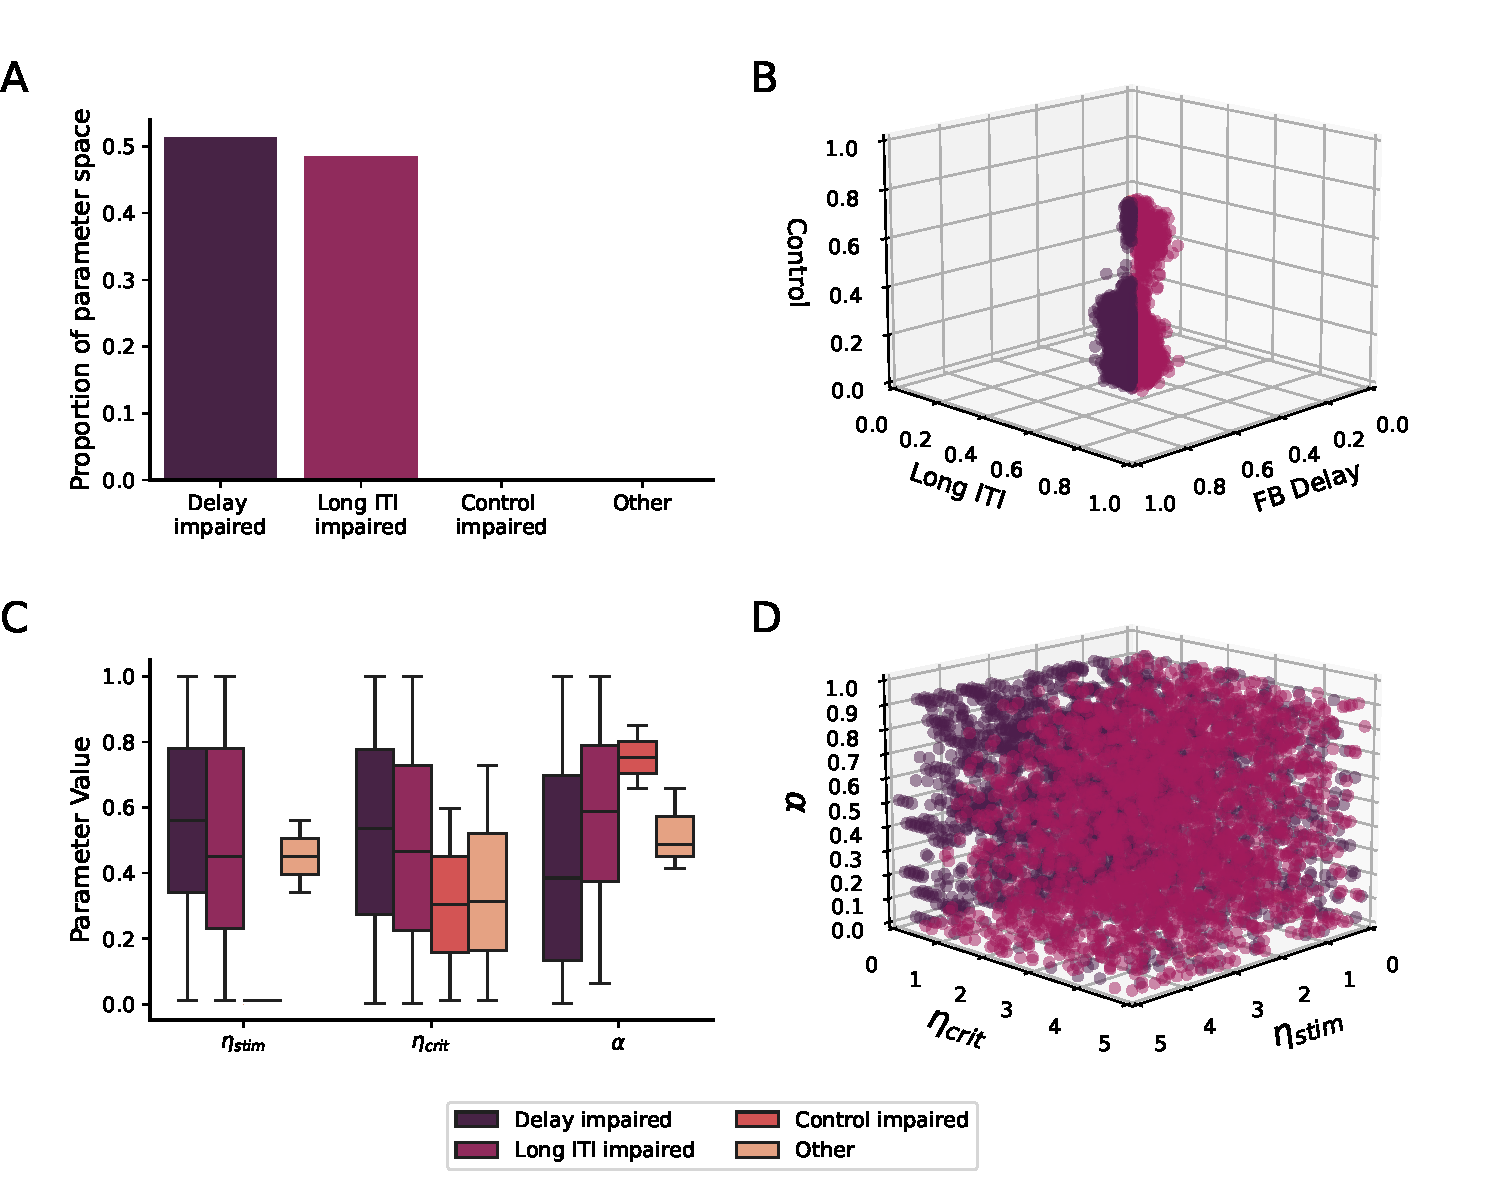
\includegraphics[width=1\textwidth]{../figures/model_working_memory.pdf}
%DIFDELCMD <   %%%
%DIFDELCMD < \caption{%
{%DIFAUXCMD
\textbf{\DIFdelFL{A:}} %DIFAUXCMD
\DIFdelFL{The proportion of parameter space where
      the time-dependent drift model predicted each of four
      qualitative patterns: (1) slower learning under
      feedback delay, (2) slower learning in the Long-ITI
      condition, (3) slower learning in the control
      condition, and (4) any other pattern. 
      %DIF <  
      }\textbf{\DIFdelFL{B:}} %DIFAUXCMD
\DIFdelFL{Simulated trials-to-criterion for each
      condition. All scores were normalized by the largest
      trials-to-criterion value within a given parameter
      set, so all axes range from zero to one. 
      %DIF <  
      }\textbf{\DIFdelFL{C:}} %DIFAUXCMD
\DIFdelFL{Boxplot of the parameter ranges leading to
      each PSP pattern. All parameter values were normalized
      by the largest value in the search range, so the
      ordinate ranges from zero to one for all parameters.
      %DIF <  
      }\textbf{\DIFdelFL{D:}} %DIFAUXCMD
\DIFdelFL{Scatter plot of the parameter ranges
      associated with each PSP pattern. 
      %DIF < 
      }\textit{\DIFdelFL{Note:}} %DIFAUXCMD
\DIFdelFL{In all panels, color indicates the PSP
      pattern.
}}
  %DIFAUXCMD
%DIFDELCMD < \label{fig:TDD_results}
%DIFDELCMD < \end{figure}
%DIFDELCMD < 

%DIFDELCMD < %%%
\DIFdel{Figure \ref{fig:TDD_results}A shows that the model
essentially always predicts that increasing the feedback
delay or the ITI have similar detrimental effects on
learning. The model makes this prediction because it assumes
that the criterion drifts during both the feedback delay and
during the ITI. So the critical variable for the model is
the time between the response on trial $n$ and the
presentation of
the stimulus on trial $n+1$. The model
assumes that the criterion drifts during this entire time,
and therefore how this interval is divided between feedback
delay and ITI is relatively unimportant to the model
predictions. 
}%DIFDELCMD < 

%DIFDELCMD < \subsubsection{Delay-sensitive learning model}
%DIFDELCMD < %%%
\DIFdel{We simulated the performance of the delay-sensitive learning
across a wide range of parameter values for $\sigma_p$ and
$\alpha$. Specifically, in the case of $\alpha$ we stepped
through every value in the interval $[0, 1]$, with a step
size of .1. In the case of $\sigma_p$, we searched over the
interval $[0.1, 5]$, with a step size of 0.1. 
}%DIFDELCMD < 

%DIFDELCMD < %%%
\DIFdel{The results are shown in Figure \ref{fig:DSL_results}. Note
that virtually all combinations of the parameter values
predict that feedback delay impairs criterial learning more
than increasing the ITI. This makes sense because Equation
\ref{eq:DSL_learning} shows that the delay-sensitive
learning model predicts that increasing the feedback delay
(i.e., increasing $t_{FD}$) will impair learning -- for any
value of $\alpha>0$. Large values of $\sigma_p$ will also
impair performance because of distortion to the percept, but
this interference will be the same in all conditions.
}%DIFDELCMD < 

%DIFDELCMD < \begin{figure}
%DIFDELCMD <   \centering
%DIFDELCMD <   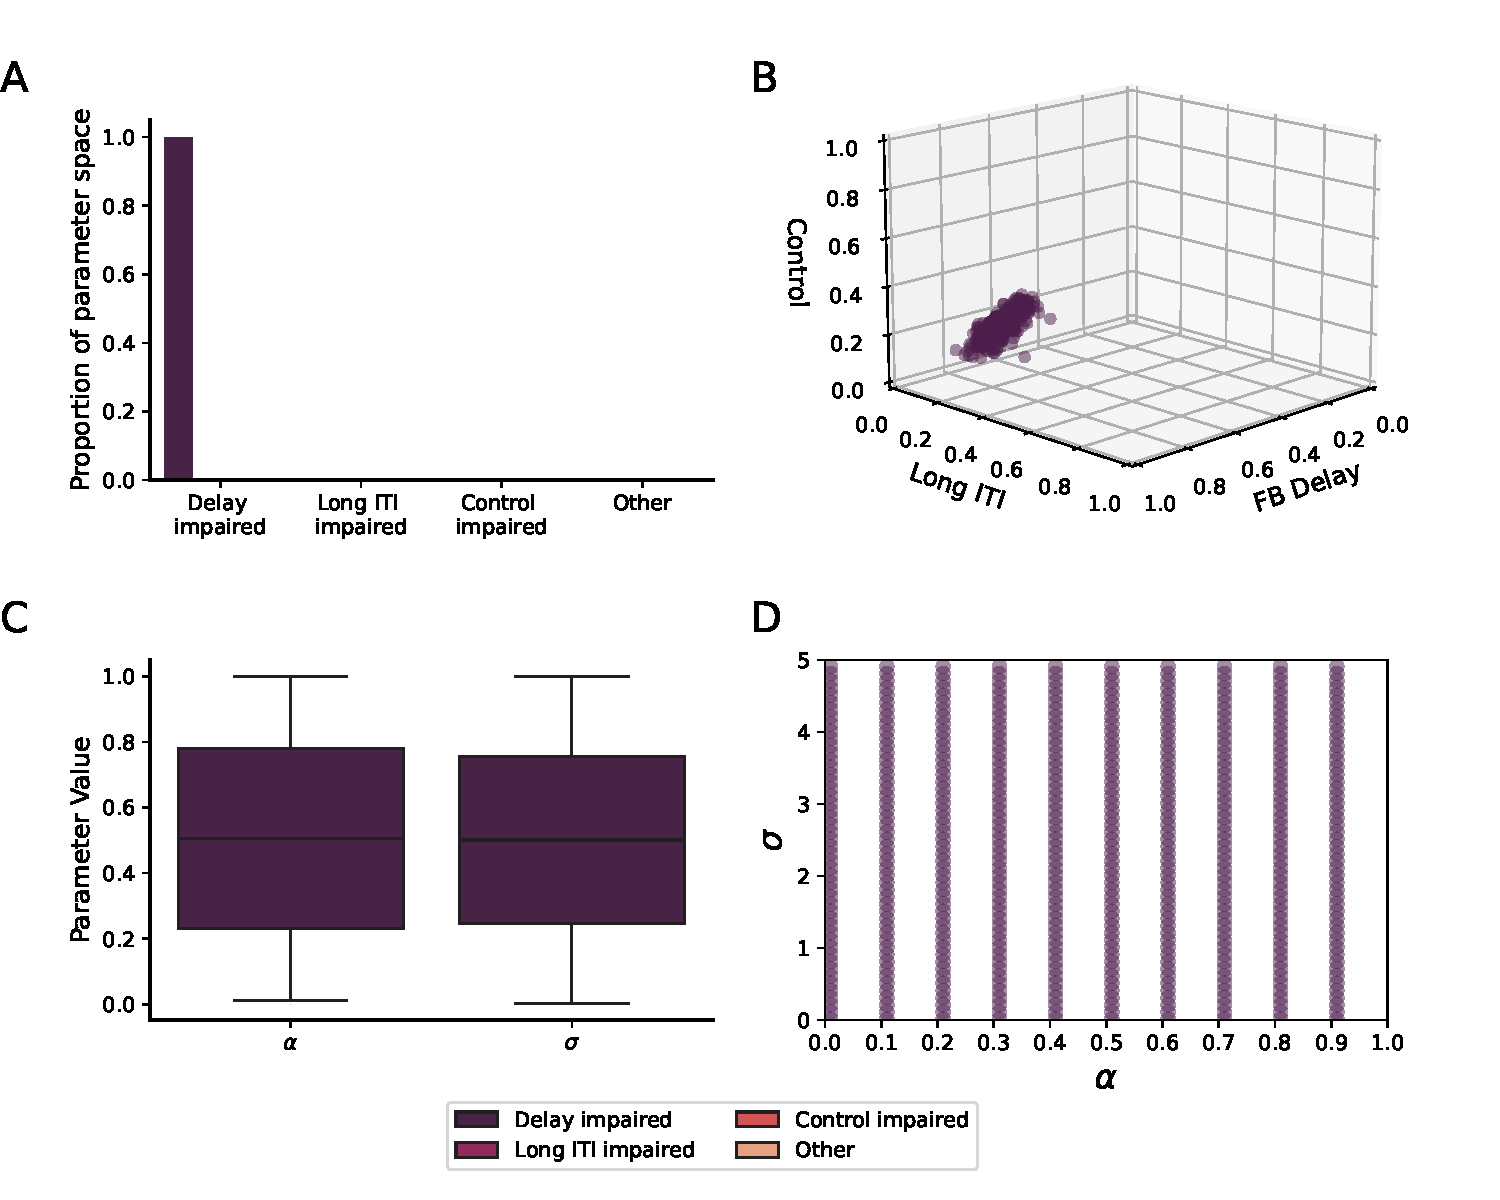
\includegraphics[width=1\textwidth]{../figures/model_procedural_supervised.pdf}
%DIFDELCMD <   %%%
%DIFDELCMD < \caption{%
{%DIFAUXCMD
\textbf{\DIFdelFL{A:}} %DIFAUXCMD
\DIFdelFL{The proportion of parameter space where
      the delay-sensitive learning model predicted each of
      four qualitative patterns: (1) slower learning under
      feedback delay, (2) slower learning in the Long-ITI
      condition, (3) slower learning in the control
      condition, and (4) any other pattern. 
      %DIF <  
      }\textbf{\DIFdelFL{B:}} %DIFAUXCMD
\DIFdelFL{Simulated trials-to-criterion for each
      condition. All scores were normalized by the largest
      trials-to-criterion value within a given parameter
      set, so all axes range from zero to one. 
      %DIF <  
      }\textbf{\DIFdelFL{C:}} %DIFAUXCMD
\DIFdelFL{Boxplot of the parameter ranges leading to
      each PSP pattern. All parameter values were normalized
      by the largest value in the search range, so the
      ordinate ranges from zero to one for all parameters.
      %DIF <  
      }\textbf{\DIFdelFL{D:}} %DIFAUXCMD
\DIFdelFL{Scatter plot of the parameter ranges
      associated with each PSP pattern. 
      %DIF < 
      }\textit{\DIFdelFL{Note:}} %DIFAUXCMD
\DIFdelFL{In all panels, color indicates the PSP
      pattern.
}}
  %DIFAUXCMD
%DIFDELCMD < \label{fig:DSL_results}
%DIFDELCMD < \end{figure}
%DIFDELCMD < 

%DIFDELCMD < \subsubsection{Reinforcement-learning model}
%DIFDELCMD < %%%
\DIFdel{We investigated the effects on performance predicted by the
reinforcement-learning model of three parameters -- the
perceptual-noise variance $\sigma^2$ and the actor and
critic learning rates (i.e., $\alpha_{actor}$ and
$\alpha_{critic}$, respectively). In the case of both
$\alpha_{actor}$ and $\alpha_{critic}$, we stepped through
every value in the interval $[0, 0.2]$, with a step size of
.01. We constrained our search over these parameters to this
interval because reinforcement-learning models are prone to
instability at very high learning rates
\mbox{%DIFAUXCMD
\parencite{SuttonBarto1998}}\hskip0pt%DIFAUXCMD
. As evidence of this, at higher
learning rates, the model failed to learn with any
consistency -- that is, in most cases, it failed to reach
the learning criterion (12 correct responses in a row)
within the allowable 200 trials. In the case of $\sigma$, we
searched over the interval $[1, 10]$, 
with a step size of 1.
As with the other models, all scores were normalized by the
largest observed value.
}%DIFDELCMD < 

%DIFDELCMD < %%%
\DIFdel{The results are described in Figure \ref{fig:RL_results}.
Note this model predicts that delayed feedback impairs
criterial learning more than a long ITI across a wide volume
of parameters settings. As can be seen in Figure
\ref{fig:RL_results}C, the only exceptions tend to occur
when the value of any of the three parameters approaches the
maximum end of the range explored. The logic here is similar
to the delay-sensitive learning model -- that is, both
models predict that increasing the feedback delay $t_{FD}$
will impair learning -- for all values of the learning rate.
}%DIFDELCMD < 

%DIFDELCMD < \begin{figure}
%DIFDELCMD <   \centering
%DIFDELCMD <   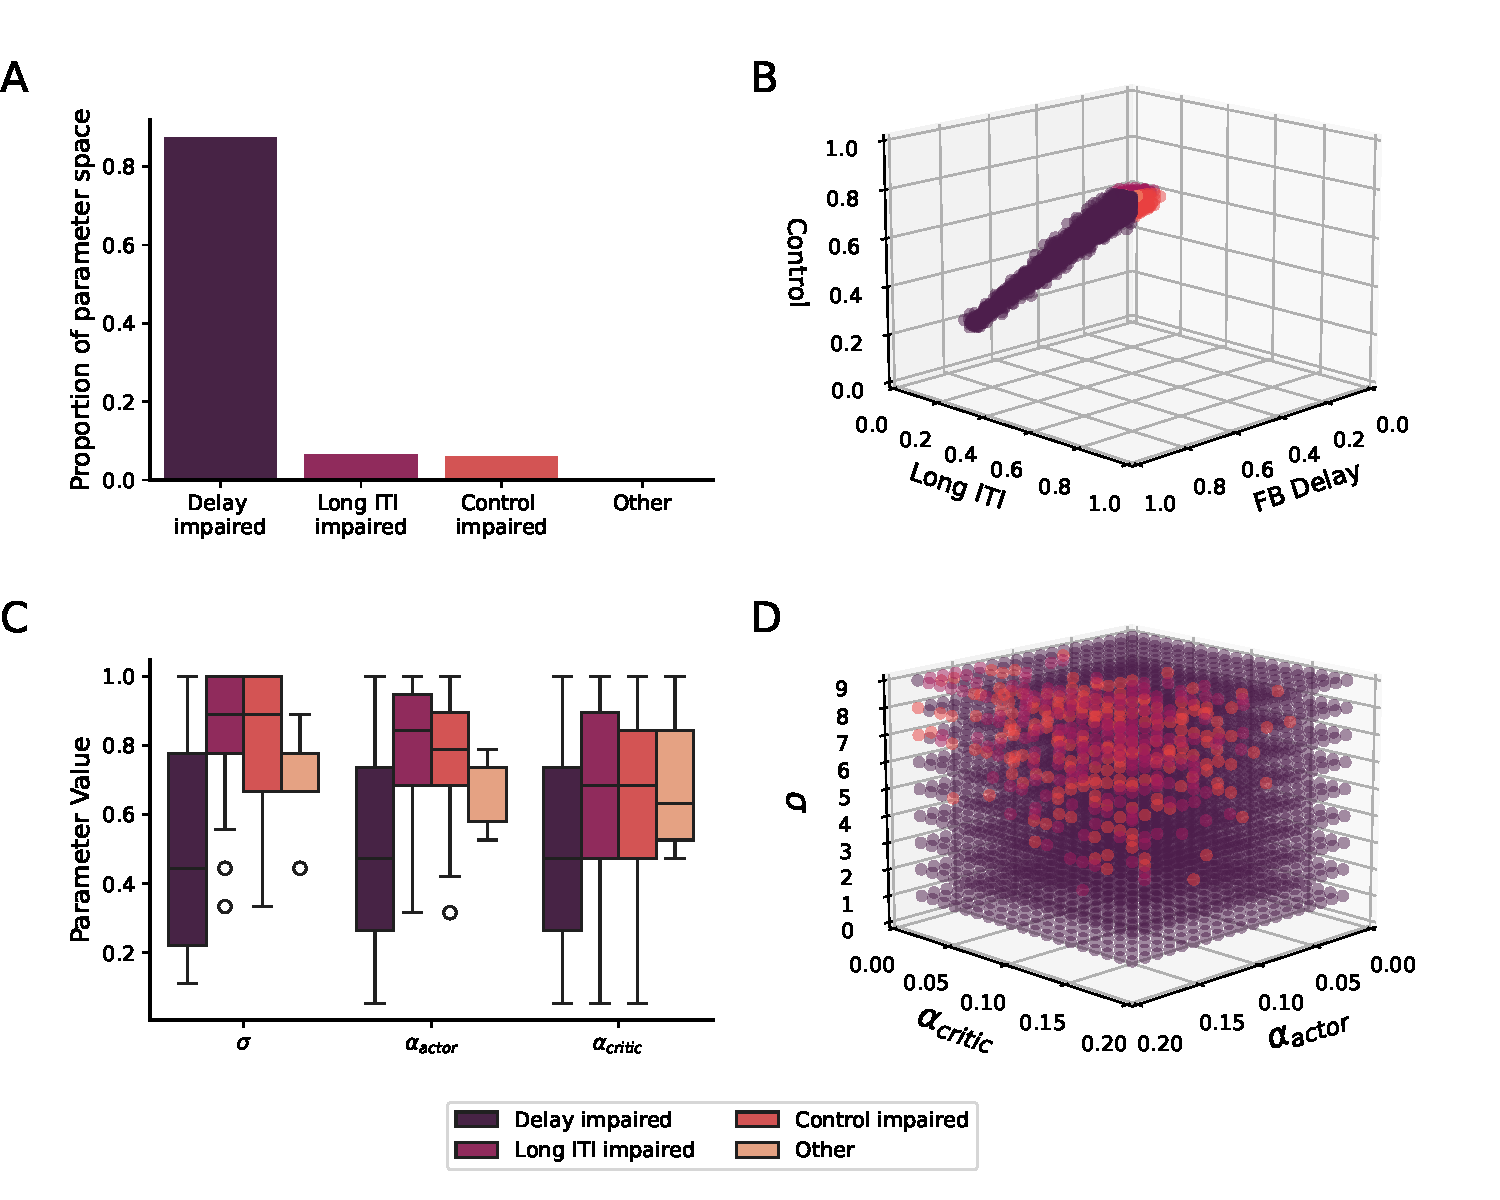
\includegraphics[width=1\textwidth]{../figures/model_procedural_reinforcement.pdf}
%DIFDELCMD <   %%%
%DIFDELCMD < \caption{%
{%DIFAUXCMD
\textbf{\DIFdelFL{A:}} %DIFAUXCMD
\DIFdelFL{The proportion of parameter space where
      the reinforcement-learning model predicted each of
      four qualitative patterns: (1) slower learning under
      feedback delay, (2) slower learning in the Long-ITI
      condition, (3) slower learning in the control
      condition, and (4) any other pattern. 
      %DIF <  
      }\textbf{\DIFdelFL{B:}} %DIFAUXCMD
\DIFdelFL{Simulated trials-to-criterion for each
      condition. All scores were normalized by the largest
      trials-to-criterion value within a given parameter
      set, so all axes range from zero to one. 
      %DIF <  
      }\textbf{\DIFdelFL{C:}} %DIFAUXCMD
\DIFdelFL{Boxplot of the parameter ranges leading to
      each PSP pattern. All parameter values were normalized
      by the largest value in the search range, so the
      ordinate ranges from zero to one for all parameters.
      %DIF <  
      }\textbf{\DIFdelFL{D:}} %DIFAUXCMD
\DIFdelFL{Scatter plot of the parameter ranges
      associated with each PSP pattern. 
      %DIF < 
      }\textit{\DIFdelFL{Note:}} %DIFAUXCMD
\DIFdelFL{In all panels, color indicates the PSP
      pattern.
    }}
  %DIFAUXCMD
%DIFDELCMD < \label{fig:RL_results}
%DIFDELCMD < \end{figure}
%DIFDELCMD < 

%DIFDELCMD < \subsubsection{Summary of modeling results}
%DIFDELCMD < %%%
\DIFdel{We investigated three criterial-learning models that make
different predictions about how increases in the }\DIFdelend \DIFaddbegin \section{Experiment 1}
\DIFadd{Experiment 1 used a one-dimensional category-learning task
to investigate how }\DIFaddend feedback delay and ITI affect \DIFdelbegin \DIFdel{learning. The time-dependent drift
model predicts that the criterion always drifts, so the
critical variable is the sum of the feedback delay and ITI.
How this sum is divided into separate feedback delay and ITI
time intervals has little effect on the model's predictions.
In contrast, the delay-sensitive learning model predicts
that feedback delays are necessarily more detrimental to
performance than increases in the ITI.  Finally, the
reinforcement-learning model also predicts that, in general,
feedback delays should impair learning more than long ITIs,
although this model is somewhat more flexible than the
delay-sensitive learning model and can account for a small
or null effect of feedback delay within a restricted region
of its parameter space. The obvious next question is how
human criterial
learningis affected by these independent
variables. Experiments 2 and 3 were designed to address this
question, and therefore also to test the predictions of the
three models.
}%DIFDELCMD < 

%DIFDELCMD < \section{Experiment 2}
%DIFDELCMD < %%%
\DIFdel{Experiment 2 investigated how feedback delay and the length
of the ITI affect criterial learning in humans. As a result,
it also provides rigorous tests of the predictions of the
time-dependent drift model, the delay-sensitive learning
model, and the reinforcement-learning model.
}%DIFDELCMD < 

%DIFDELCMD < %%%
\DIFdelend \DIFaddbegin \DIFadd{criterial
learning. }\DIFaddend The stimuli in \DIFdelbegin \DIFdel{Experiment 2 }\DIFdelend \DIFaddbegin \DIFadd{this experiment }\DIFaddend were circular
sine-wave gratings that varied across trials in bar width
and bar orientation. These stimuli were divided into two
categories according to their value on one of the two
dimensions. In other words, the optimal strategy was to set
a response criterion on the single relevant dimension, and
then choose a categorization response based on whether the
value of the presented \DIFdelbegin \DIFdel{stimuli
}\DIFdelend \DIFaddbegin \DIFadd{stimulus }\DIFaddend on this dimension was larger
or smaller than the criterion value.  \DIFdelbegin %DIFDELCMD < 

%DIFDELCMD < %%%
\DIFdelend The experiment
isolated criterial learning by (1) explicitly instructing
participants \DIFdelbegin \DIFdel{on }\DIFdelend \DIFaddbegin \DIFadd{about }\DIFaddend the relevant stimulus dimension and rule
structure (e.g., thick bars are ``A'', thin bars are ``B''),
and (2) eliminating \DIFaddbegin \DIFadd{all }\DIFaddend variability along the irrelevant
stimulus dimension. In other words, the instructions
identified the relevant stimulus dimension, and as a result,
the only learning required was criterial learning. 

\DIFaddbegin \DIFadd{Each participant practiced each of 14 one-dimensional
category-learning tasks, or problems, until they responded
correctly on 9 of the 10 previous trials, at which point the
problem changed. The 14 different category structures are
described in Figure \ref{fig_design_exp_1_space}. The
relevant dimension was bar thickness in problems 1 -- 7 and
bar angle in problems 8 -- 14. Each problem included stimuli
in two distinct clusters that varied over a restricted range
of the relevant dimension. Critically, the optimal criterion
value varied from problem-to-problem with respect to its
position within the stimulus range. For example, for some
problems the optimal criterion was below the midpoint of the
range and for other problems it was above the midpoint.
Feedback delay and ITI were varied across three conditions.
In the Delayed-Feedback condition, feedback was delayed
after the observer responded (by 3.5 s) and the ITI was
short (500 ms). In the Long-ITI condition, the feedback
delay was short (500 ms) and the ITI was long (3.5 s).
Finally, in the Control condition, feedback delay and the
ITI were both 500 ms.
}

\begin{figure}
  \centering
  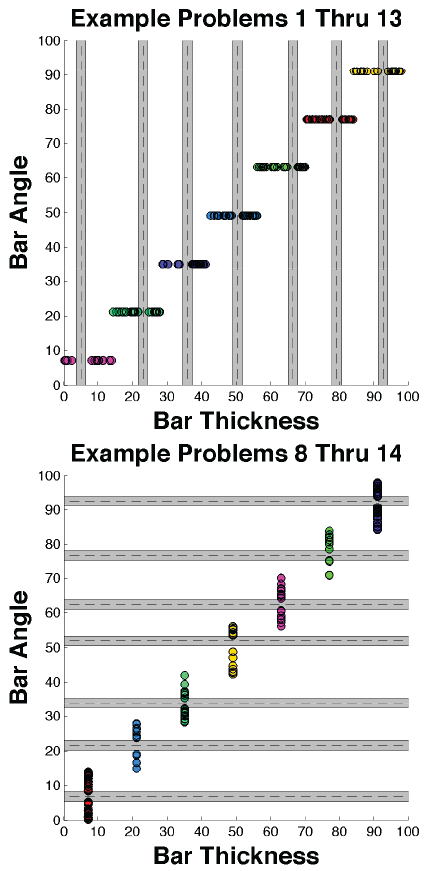
\includegraphics[width=.5\textwidth]{../figures/fig_design_exp_1_space.png}
  \caption{
      \DIFaddFL{Category sample space. Different colors represent
      different category problems. Dashed lines are category
      boundaries (criterion) and the surrounding solid lines
      mark the no-stimulus region in which no stimuli were
      sampled.
}}
  \label{fig_design_exp_1_space}
\end{figure}

\DIFaddend \subsection{Method}

\subsubsection{Apparatus}
All experiments were performed in a dimly lit room.
Participants sat approximately 24'' from a 17'' $\times$
11'' monitor running at a resolution of 1680 $\times$ 1050
pixels. Participants made category judgments by pressing the
`d' or `k' keys on a standard computer keyboard for `A' or
`B' choices, respectively. Stickers with bold print `A' or
`B' were placed on the appropriate keys.

\subsubsection{Stimuli and Categories}
Stimuli were circular sine-wave gratings that varied in bar
width and bar orientation, drawn from various 1-dimensional
uniform distributions specific to the current category
problem. We first defined an arbitrary 2-dimensional
$[0-100,0-100]$ stimulus space, and then split each
dimension of this space into 7 bins of width 14 units each.
Each $(x,y)$ pair from this arbitrary stimulus space was
converted to a grating according to the nonlinear
transformations defined by
\textcite{treutwein1989perceptual}, which roughly equate the
salience of each dimension\DIFdelbegin \DIFdel{(for }\DIFdelend \DIFaddbegin \DIFadd{. For }\DIFaddend details, see also
\textcite{CrossleyAshby2015}\DIFdelbegin \DIFdel{)}\DIFdelend .

The structure of the various criterial-learning tasks is
illustrated in Figure \ref{fig_design_exp_1_space}. Each
criterial-learning problem was created by first \DIFdelbegin \DIFdel{randomly
}\DIFdelend selecting a
relevant dimension\DIFdelbegin \DIFdel{, and then randomly selecting
}\DIFdelend \DIFaddbegin \DIFadd{. This was spatial frequency for the
problems 1 through 7 and orientation for problems 8 through
14. We then randomly selected }\DIFaddend one of the 7 bins defined on
that dimension. Each bin was also associated with a
corresponding unique value on the irrelevant dimension. We
buffered the to-be-learned response criterion by 10\% of
total bin width on either side with a no-stimulus region.
Random uniform samples from the remaining eligible region of
each bin were then selected and presented to the participant
until 9 correct responses out of any 10 responses in a row
advanced the participant to the next problem. Note that
every category problem was a simple one-dimensional rule in
which optimal accuracy was 100\%.  Note also that the
relative location of the optimal response criterion varied
across problems.

\DIFdelbegin %DIFDELCMD < \begin{figure}
%DIFDELCMD <   \centering
%DIFDELCMD <   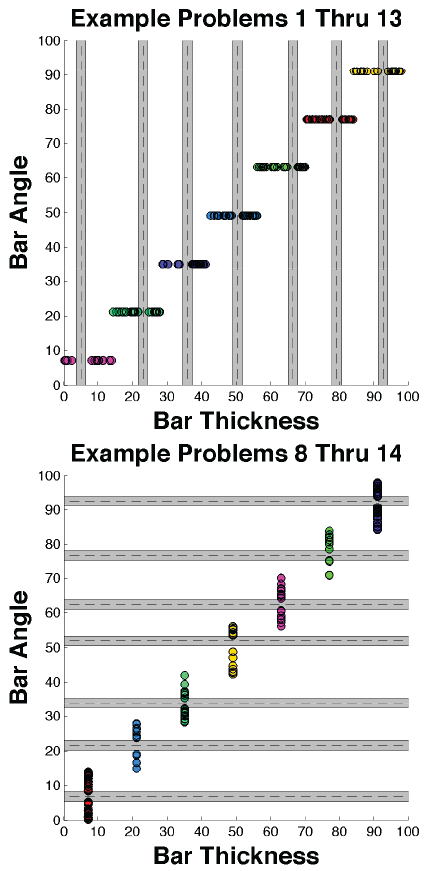
\includegraphics[width=.5\textwidth]{../figures/fig_design_exp_1_space.png}
%DIFDELCMD <   %%%
%DIFDELCMD < \caption{%
{%DIFAUXCMD
\DIFdelFL{Category sample space. Different colors represent
      different category problems. Dashed lines are category
      boundaries (criterion) and the surrounding solid lines
      mark the no-stimulus region in which no stimuli were
      sampled.
}}
  %DIFAUXCMD
%DIFDELCMD < \label{fig_design_exp_1_space}
%DIFDELCMD < \end{figure}
%DIFDELCMD < 

%DIFDELCMD < %%%
\DIFdelend \subsubsection{Procedure}
There were three conditions (described in detail in Table
\ref{conditions_exp_1}). In the Delayed-Feedback condition,
feedback was delayed 3.5 s after the response and the ITI
was 0.5 s. In the Long-ITI condition, feedback was delayed
0.5 s after the response and the ITI was 3.5 s. Finally, in
the Control condition, feedback was delayed 0.5 s after the
response and the ITI was 0.5 s.

Each participant completed a series of one-dimensional
category-learning tasks or problems, which are described in
Figure \ref{fig_design_exp_1_space}. Each problem included
stimuli in two distinct clusters that varied over a
restricted range of the relevant dimension. Critically, the
optimal criterion value varied from problem-to-problem with
respect to its position within this range. For example, for
some problems the optimal criterion was below the midpoint
of the range and for other problems it was above the
midpoint. 

Participants were explicitly told the relevant dimension for
each problem, as well as the generic response mapping (e.g.,
thick bars = ``A'', thin bars = ``B''). Figure
\ref{fig:trial} shows the structure of an example trial,
along with an example of a typical category structure. All
trials in every condition included a 500 ms fixation cross,
a response-terminated stimulus, a circular white-noise mask,
corrective feedback, and an inter-trial interval (ITI) that
varied according to condition. The text `Correct' was
displayed in centered, large green font after correct
responses, and the text `Incorrect' was displayed in
centered, large red font after incorrect responses.

Participants practiced each problem until they responded
correctly on 9 of the previous 10 trials. At this point, the
problem changed. Each participant completed as many problems
as possible in 512 trials or until they had been in the lab
for 60 minutes (including time to acquire consent and give
instructions), at which point the session was terminated.

\begin{figure}
  \centering
  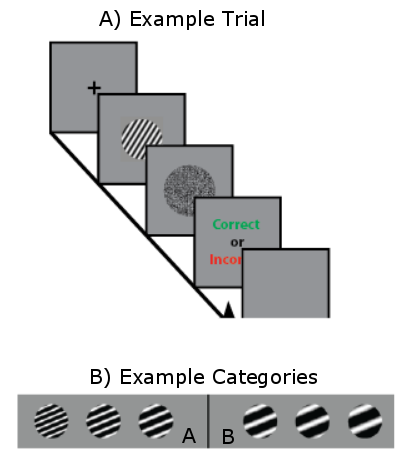
\includegraphics[width=.5\textwidth]{../figures/fig_design_exp_1.png}
  \caption{
      Example trial and category problem. A) Events that
      occurred on each trial. B) An example of a typical
      category structure.
}
  \label{fig:trial}
\end{figure}

\begin{table}
    \caption{
        Durations (in s) of Trial Events in each Condition.
    }
    \label{conditions_exp_1}
    \begin{tabular}{c|cccc}
        Conditions & Stim & Mask & FB & ITI \\[0.5ex] \hline Control & RT & 0.5 &
        1.0 & 0.5 \\[0.5ex]
        \\[-1.5ex] Delayed Feedback &
        RT & 3.5 & 1.0 & 0.5 \\[0.5ex]   Long ITI & RT & 0.5 & 1.0 & 3.5
        \\[0.5ex]
    \end{tabular}
\end{table}

\subsubsection{Participants}
Fifty-nine participants participated in Experiment \DIFdelbegin \DIFdel{2. }\DIFdelend \DIFaddbegin \DIFadd{1. }\DIFaddend All
were UCSB undergraduates and received course credit for
their participation. All had normal or corrected to normal
vision. We randomly assigned each participant to one of
three conditions (target $N>16$ per condition based on
similar previous research): Delayed Feedback ($N = 20$);
Long ITI ($N = 21$), Control ($ N = 17$). All participants
gave written informed consent before participating in the
study. All experimental protocols were approved by the
University of California at Santa Barbara Human Subjects
Committee in the Office of Research Development and
Administration.

\subsection{Results}
\DIFdelbegin \DIFdel{Figure \ref{fig_gmm_hist_1} shows a }\DIFdelend \DIFaddbegin \DIFadd{Both panels of Figure \ref{fig_mm_hist_1} show the same
}\DIFaddend relative frequency histogram of the trials-to-criterion
\DIFdelbegin \DIFdel{observed across all three }\DIFdelend \DIFaddbegin \DIFadd{collapsed across all participants and }\DIFaddend conditions. The
histogram shows that the majority of participants were able
to learn each problem on average in less than 100 trials.
However, this histogram also shows that a subset of
participants required many more trials to learn each
problem. Given that \DIFdelbegin \DIFdel{each problem is very simple
and that }\DIFdelend \DIFaddbegin \DIFadd{participants were explicitly instructed
about }\DIFaddend the relevant dimension of each problem\DIFdelbegin \DIFdel{is
explicitly instructed to participants, it is }\DIFdelend \DIFaddbegin \DIFadd{, the task was
relatively simple and as a result, it seems }\DIFaddend likely that the
participants \DIFdelbegin \DIFdel{in }\DIFdelend \DIFaddbegin \DIFadd{represented by }\DIFaddend the tails of this distribution
did not pay attention to the instructions, were not
motivated to learn the task, were distracted by other
factors, or should be considered outliers for some other
reason. \DIFaddbegin \DIFadd{In our experience, it is not unusual for a small
subset of participants to perform very poorly in experiments
of this kind. This typically reflects a lack of engagement
or misunderstanding of the task instructions rather than an
inability to perform the task itself.
}\DIFaddend 

\begin{figure}
  \centering
  \DIFdelbeginFL %DIFDELCMD < 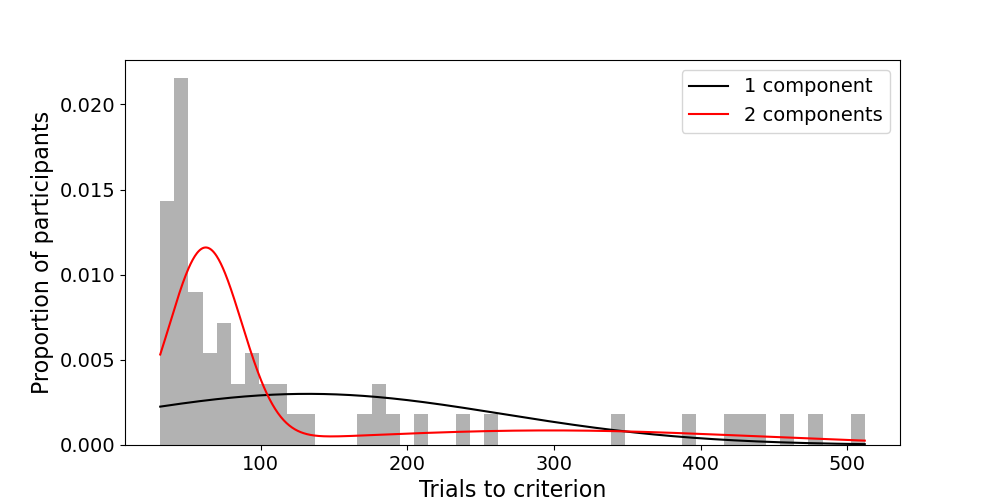
\includegraphics[width=.8\textwidth]{../figures/fig_exp_1_gmm.png}
%DIFDELCMD <   %%%
\DIFdelendFL \DIFaddbeginFL 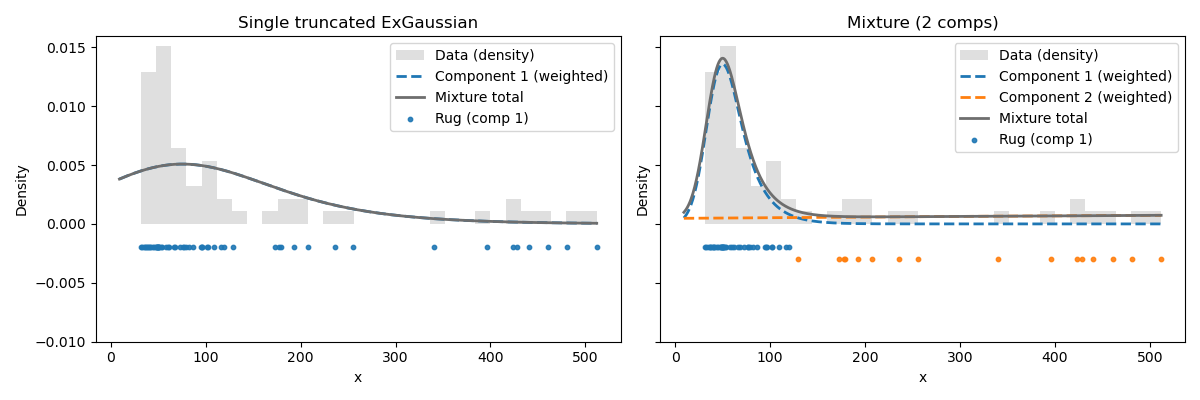
\includegraphics[width=1\textwidth]{../figures/fig_exp_1_mm_trunc_exgauss_compare.png}
  \DIFaddendFL \caption{
      Relative frequency histogram of the
      trials-to-criterion \DIFdelbeginFL \DIFdelFL{observed }\DIFdelendFL \DIFaddbeginFL \DIFaddFL{collapsed }\DIFaddendFL across all three
      conditions \DIFaddbeginFL \DIFaddFL{and participants }\DIFaddendFL in Experiment \DIFdelbeginFL \DIFdelFL{2. }\DIFdelendFL \DIFaddbeginFL \DIFaddFL{1. }\DIFaddendFL The \DIFdelbeginFL \DIFdelFL{black line are }\DIFdelendFL \DIFaddbeginFL \DIFaddFL{left
      panel shows }\DIFaddendFL the \DIFdelbeginFL \DIFdelFL{predictions of }\DIFdelendFL \DIFaddbeginFL \DIFaddFL{best-fitting single ExGaussian
      distribution and }\DIFaddendFL the \DIFaddbeginFL \DIFaddFL{right panel shows the
      }\DIFaddendFL best-fitting \DIFdelbeginFL \DIFdelFL{one-component Gaussian
      Mixture Model to these data}\DIFdelendFL \DIFaddbeginFL \DIFaddFL{two-component ExGaussian mixture model.
      In the right panel}\DIFaddendFL , \DIFdelbeginFL \DIFdelFL{whereas }\DIFdelendFL the \DIFdelbeginFL \DIFdelFL{red }\DIFdelendFL \DIFaddbeginFL \DIFaddFL{blue dashed }\DIFaddendFL line \DIFdelbeginFL \DIFdelFL{represents }\DIFdelendFL \DIFaddbeginFL \DIFaddFL{is }\DIFaddendFL the \DIFdelbeginFL \DIFdelFL{best fit of }\DIFdelendFL \DIFaddbeginFL \DIFaddFL{first
      higher performance component, }\DIFaddendFL the \DIFdelbeginFL \DIFdelFL{two-component Gaussian
      Mixture Model}\DIFdelendFL \DIFaddbeginFL \DIFaddFL{orange dashed line
      is the second lower performance component}\DIFaddendFL .       The
      \DIFaddbeginFL \DIFaddFL{gray solid line is the mixture distribution that
      combines these two components. Rug plots along the
      x-axes show the individual data      colored by their
      assignment to either the higher or lower performance
      component. The }\DIFaddendFL two-component model provided a
      significantly better fit according to AIC, BIC, and a
      likelihood ratio test.
}
  \DIFdelbeginFL %DIFDELCMD < \label{fig_gmm_hist_1}
%DIFDELCMD < %%%
\DIFdelendFL \DIFaddbeginFL \label{fig_mm_hist_1}
\DIFaddendFL \end{figure}

%DIF <  AIC for 1 component: 735.7652217198266
%DIF <  AIC for 2 components: 662.8095009936025
%DIF <  
%DIF <  BIC for 1 component: 739.8861077409194
%DIF <  BIC for 2 components: 673.1117160463345
%DIF < 
%DIF <  LRT statistic: 78.95572072622417
%DIF <  Degrees of freedom: 3
%DIF <  P-value: 5.140608761896481e-17
\DIFdelbegin %DIFDELCMD < 

%DIFDELCMD < %%%
\DIFdel{We }\DIFdelend \DIFaddbegin \DIFadd{We identified and removed from further analyses these
outlier participants using the following algorithm. First,
we }\DIFaddend modeled the distribution shown in Figure
\DIFdelbegin \DIFdel{\ref{fig_gmm_hist_1} using a Gaussian mixture model with two components}\DIFdelend \DIFaddbegin \DIFadd{\ref{fig_mm_hist_1} using a mixture of two ExGaussian
distributions,}\footnote{\DIFadd{The ExGaussian is the distribution
of the sum of two independent random variables -- one with
an exponential distribution and one with a normal or
Gaussian distribution.}} \DIFadd{each truncated to the range of
possible trials-to-criterion values (i.e., $[9,512]$)}\DIFaddend . The
first \DIFdelbegin \DIFdel{component captured }\DIFdelend \DIFaddbegin \DIFadd{distribution or component was assumed to model
performance of }\DIFaddend participants with a relatively low mean
number of trials-to-criterion, \DIFdelbegin \DIFdel{while }\DIFdelend \DIFaddbegin \DIFadd{whereas }\DIFaddend the second component
\DIFdelbegin \DIFdel{identified outliers according to the above
rationale. We }\DIFdelend \DIFaddbegin \DIFadd{was assumed to identify outlier participants. We estimated
parameters of this model using maximum likelihood estimation
with proper normalization on the tasks bounded support and
compared them via the AIC and BIC goodness-of-fit
statistics, and a parametric bootstrap likelihood-ratio
test. We then }\DIFaddend compared the fit of this two-component model
to a single-component \DIFdelbegin \DIFdel{model using the Akaike Information
Criterion (AIC ) and Bayesian Information Criterion (BIC)}\DIFdelend \DIFaddbegin \DIFadd{ExGaussian model using AIC and BIC}\DIFaddend ,
both of which indicated a better fit for the two-component
model (\DIFdelbegin \DIFdel{AIC: 662.81 vs. 735.77;
BIC: 673.11 vs. 739.89). Additionally, a likelihood ratio test }\DIFdelend \DIFaddbegin \DIFadd{$\mathrm{AIC}_1=692.15$ vs. $\mathrm{AIC}_2=652.81$;
$\mathrm{BIC}_1=698.33$ vs. $\mathrm{BIC}_2=667.23$). The
bootstrap likelihood-ratio test also }\DIFaddend confirmed that the
two-component model provided a significantly better fit than
the one-component model (\DIFdelbegin \DIFdel{$\chi^2(3) = 78.96$, $p < .001$). Outlier participants were then }\DIFdelend \DIFaddbegin \DIFadd{$D=42.84$, $p_{\text{boot}}\approx
.01$). Next, for each participant, we used the
best-fitting two component model to compute the likelihood
that their performance was best described by each component.
Participants whose data were estimated to most likely belong
to the low-performance distribution were classified as
outliers and }\DIFaddend excluded from further analysis. After making
these \DIFdelbegin \DIFdel{exlcusions}\DIFdelend \DIFaddbegin \DIFadd{exclusions}\DIFaddend , we were left with the following sample
sizes:  Control condition ($ N = 11$); Delayed-Feedback
condition ($N = 14$); Long-ITI condition ($N = 17$).

Figure \ref{fig_exp_1_t2c}A shows the mean
trials-to-criterion \DIFaddbegin \DIFadd{for all non-excluded participants }\DIFaddend in
each condition of Experiment \DIFdelbegin \DIFdel{2.  }\DIFdelend \DIFaddbegin \DIFadd{1.  }\DIFaddend A one-way ANOVA revealed a
significant effect of condition ($F(2, 39) = 6.17$, $p <
.01$, $\eta^2 = .24$) and planned comparisons revealed that
performance in the Delayed-Feedback condition was
significantly worse than in either the Control condition
($t(23.00) = 2.70$, $p < .05$\DIFaddbegin \DIFadd{, $d=1.06$}\DIFaddend ) or the Long-ITI
condition ($t(20.96) = 2.94$, $p < .01$\DIFaddbegin \DIFadd{, $d=1.10$}\DIFaddend ).
Performance in the Control and Long-ITI conditions did not
differ significantly from each other (\DIFdelbegin \DIFdel{$t(17.99) = 0.22$}\DIFdelend \DIFaddbegin \DIFadd{$t(17.99) = .22$}\DIFaddend , $p
= .83$\DIFdelbegin \DIFdel{).
}\DIFdelend \DIFaddbegin \DIFadd{, $d=.09$). }\footnote{\DIFadd{Including the excluded outliers
in these analyses eliminates the difference between
conditions.}}
\DIFaddend 

%DIF <    Source  ddof1  ddof2         F     p-unc       np2
%DIF <  0    cnd      2     39  6.171331  0.004693  0.240398
%DIF < 
%DIF <            A          B         T        dof     p-unc
%DIF <  0     Delay   Long ITI  2.938217  20.959026  0.007864
%DIF <  1     Delay  Short ITI  2.701083  22.997274  0.012748
%DIF <  2  Long ITI  Short ITI  0.219862  17.987044  0.828454
\DIFdelbegin %DIFDELCMD < 

%DIFDELCMD < %%%
\DIFdelend Figure \ref{fig_exp_1_t2c}B shows the mean number of
problems solved in each condition of Experiment \DIFdelbegin \DIFdel{2. }\DIFdelend \DIFaddbegin \DIFadd{1. }\DIFaddend A one-way
ANOVA revealed a significant effect of condition ($F(2, 39)
= 5.77$, $p < .01$, $\eta^2 = .23$). Planned comparisons
revealed that performance in the Delayed-Feedback condition
was significantly worse than in the Control condition
($t(18.54) = -3.28$, $p < .01$\DIFaddbegin \DIFadd{, $d=-1.21$}\DIFaddend ) and worse than in
the Long ITI condition ($t(21.60) = -2.14$, $p < .05$\DIFaddbegin \DIFadd{,
$-.80$}\DIFaddend ).  Performance in the Control and Long-ITI conditions
did not differ significantly from each other ($t(25.97) =
-1.50$, $p=.15$\DIFaddbegin \DIFadd{, $d=-.53$}\DIFaddend ).

%DIF <    Source  ddof1  ddof2         F     p-unc       np2
%DIF <  0    cnd      2     39  5.766358  0.006399  0.228223
%DIF <  
%DIF <            A          B         T        dof     p-unc
%DIF <  0     Delay   Long ITI -2.143777  21.590392  0.043579
%DIF <  1     Delay  Short ITI -3.277500  18.536603  0.004061
%DIF <  2  Long ITI  Short ITI -1.501591  25.965920  0.145267
\DIFdelbegin %DIFDELCMD < 

%DIFDELCMD < %%%
\DIFdelend \begin{figure}
  \centering
  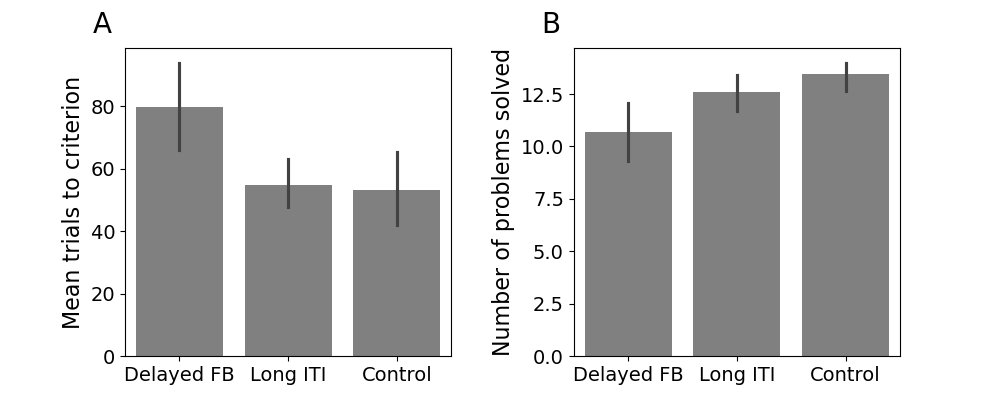
\includegraphics[width=.8\textwidth]{../figures/fig_exp_1_t2c.png}
    \caption{
        \textbf{A}: Mean \DIFdelbeginFL \DIFdelFL{trials to criterion }\DIFdelendFL \DIFaddbeginFL \DIFaddFL{trials-to-criterion }\DIFaddendFL in each
        condition of Experiment \DIFdelbeginFL \DIFdelFL{2. }\DIFdelendFL \DIFaddbeginFL \DIFaddFL{1. }\DIFaddendFL Error bars are standard
        errors of the mean.
        %
        \textbf{B}: Mean number of problems solved in each
        condition of Experiment \DIFdelbeginFL \DIFdelFL{2. }\DIFdelendFL \DIFaddbeginFL \DIFaddFL{1. }\DIFaddendFL Error bars are standard
        errors of the mean.
}
  \label{fig_exp_1_t2c}
\end{figure}

\DIFdelbegin %DIFDELCMD < \section{Experiment 3}
%DIFDELCMD < %%%
\DIFdel{Experiment 3 was designed to reinforce the findings of Experiment }\DIFdelend \DIFaddbegin \section{Experiment 2}
\DIFadd{According to a popular model of one-dimensional rule-based
category learning \mbox{%DIFAUXCMD
\parencite[i.e.,
COVIS;][]{AshbyCOVIS1998}}\hskip0pt%DIFAUXCMD
, successful learning requires at
least three separate cognitive processes: selecting a rule
for testing, switching from one candidate rule to another
(following negative feedback), and criterial learning.
Experiment 1 isolated criterial learning from this set.
Experiment }\DIFaddend 2 \DIFdelbegin \DIFdel{by using the same design but with stimuli that
have binary-valued dimensions, thereby eliminating }\DIFdelend \DIFaddbegin \DIFadd{complements Experiment 1 by using a task that
required rule selection and rule switching, but no }\DIFaddend criterial
learning. 
\DIFdelbegin \DIFdel{Unlike }\DIFdelend \DIFaddbegin 

\DIFaddend Experiment 2 \DIFdelbegin \DIFdel{, we did not explicitly
instruct participants on the relevant stimulus dimension in Experiment 3.  While Experiment 2 isolated criterial
learning from rule selection and rule switching,
this
experiment isolates rule selection and switching from
criterial learning
. Therefore, Experiment 3 was }\DIFdelend \DIFaddbegin \DIFadd{used colored geometric figures as stimuli,
which varied across trials on six binary dimensions (i.e.,
see Figure \ref{fig_design_exp_2}B). As in Experiment 1,
only one dimension was relevant. Unlike Experiment 1,
however, participants were given no instruction as to which
dimension was relevant. Therefore, this task required
participants to discover the relevant dimension. However,
after this dimension was identified, no criterial learning
was required because each stimulus always had one of two
possible values on the relevant dimension and participants
were instructed that there were two categories. Experiment 2
was therefore }\DIFaddend designed to test whether the impaired learning
that we observed in Experiment \DIFdelbegin \DIFdel{2 }\DIFdelend \DIFaddbegin \DIFadd{1 }\DIFaddend when the feedback was
delayed can be attributed principally to criterial learning
or whether it could be due to some more general
category-learning process.

\subsection{Method}

\subsubsection{Apparatus}
The apparatus was the same as in Experiment \DIFdelbegin \DIFdel{2.
}\DIFdelend \DIFaddbegin \DIFadd{1.
}\DIFaddend 

\subsubsection{Stimuli and Categories}
The stimuli consisted of colored geometric figures presented
on a colored background. These varied across six binary
dimensions: the number of items (either one or two), the
size of the items (small or large), the color of the items
(yellow or blue), the shape of the items (circle or square),
the texture of the background (smooth or rough), and the
orientation of the background (horizontal or tilted by 20
degrees). This combination resulted in a total of 64 unique
stimuli ($2^6$). An example trial and stimuli are shown in
Figure \ref{fig_design_exp_2}. In all conditions, the order
of stimulus presentation was fully randomized for each
participant, and the relevant dimension for each problem was
selected randomly without replacement from the set of six
dimensions.

\begin{figure}
  \centering
  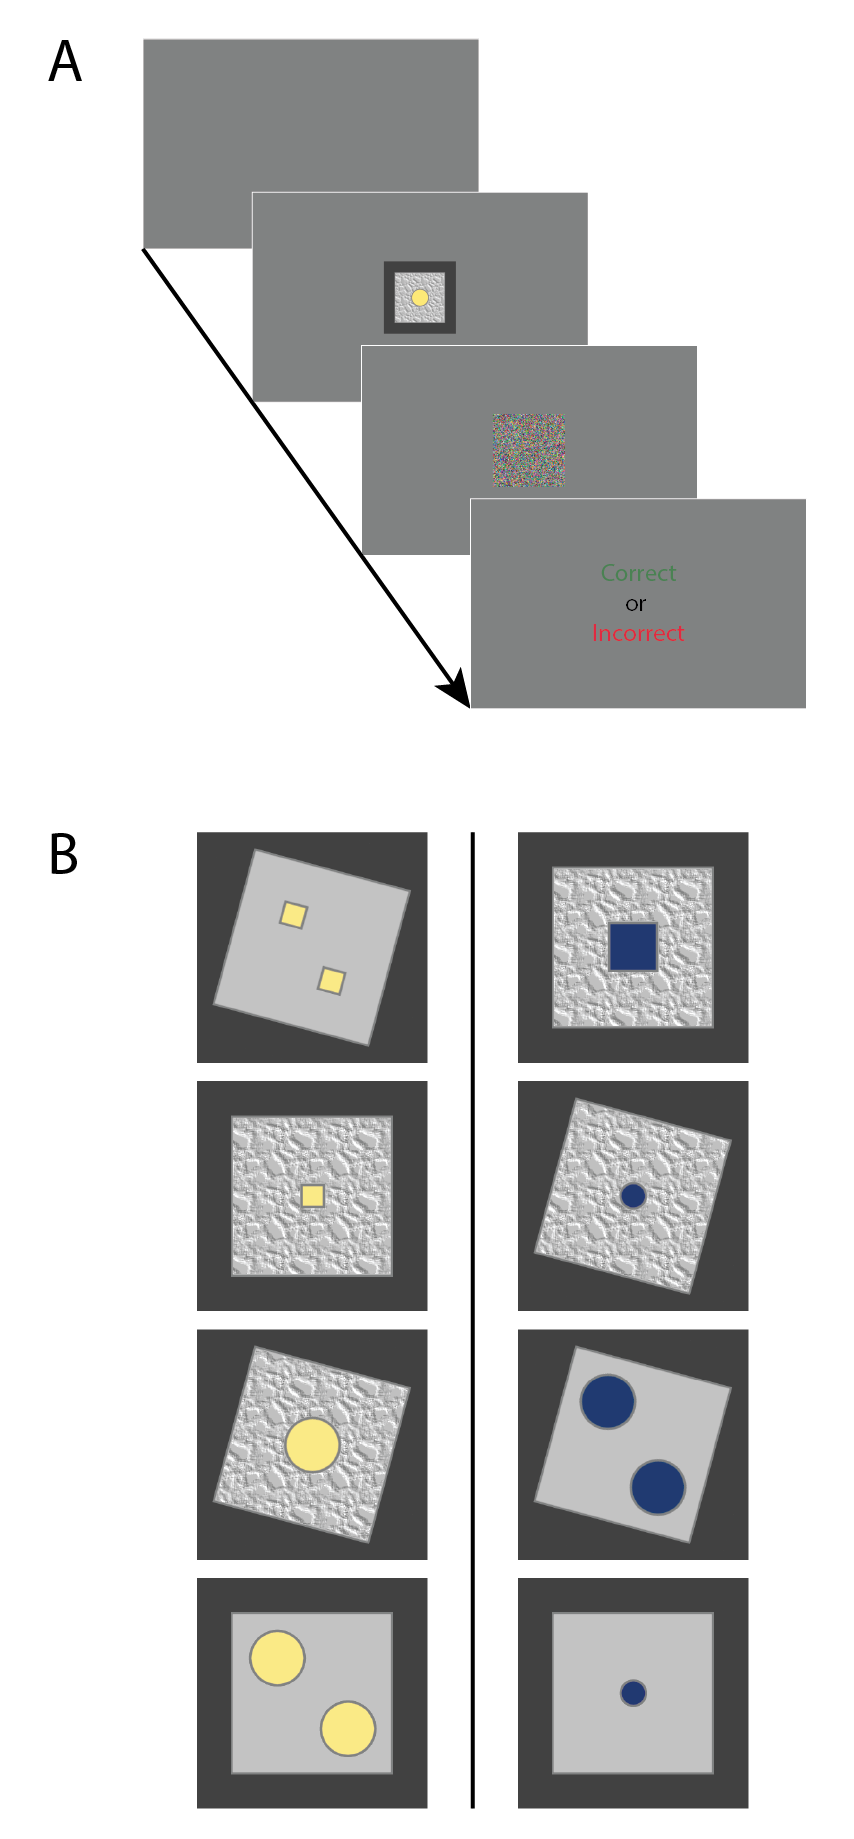
\includegraphics[width=.5\textwidth]{../figures/fig_design_exp_2.png}
  \caption{
      \textbf{A:} An example trial from Experiment \DIFdelbeginFL \DIFdelFL{3.
      }\DIFdelendFL \DIFaddbeginFL \DIFaddFL{2.
      }\DIFaddendFL \textbf{B:} Eight example stimuli (out of 64 total
      stimuli) from a possible one-dimensional rule problem.
      In this case the correct rule is `A' if the shape
      color is yellow and `B' if the shape color is blue.
      The solid line represents the category boundary.
}
  \label{fig_design_exp_2}
\end{figure}

\subsubsection{Procedure}
Participants received detailed instructions about the task.
However, unlike in Experiment \DIFdelbegin \DIFdel{2}\DIFdelend \DIFaddbegin \DIFadd{1}\DIFaddend , they were not informed of
the relevant dimension or the correct rule. The trial timing
for the Delayed-Feedback and Long-ITI conditions in
Experiment \DIFdelbegin \DIFdel{3 }\DIFdelend \DIFaddbegin \DIFadd{2 }\DIFaddend were the same as in Experiment \DIFdelbegin \DIFdel{2. Experiment 3
}\DIFdelend \DIFaddbegin \DIFadd{1. Experiment 2
}\DIFaddend did not include a condition that was analogous to the
Control condition of Experiment \DIFdelbegin \DIFdel{2. }\DIFdelend \DIFaddbegin \DIFadd{1. }\DIFaddend Participants practiced
each problem until they responded correctly on 12
consecutive trials. At this point, the problem changed. Each
participant completed as many problems as possible in 600
trials or until they had been in the lab for 30 minutes
(including time to acquire consent and give instructions),
at which point the session was terminated.

\subsubsection{Participants}
Thirty-four participants participated in Experiment \DIFdelbegin \DIFdel{3. }\DIFdelend \DIFaddbegin \DIFadd{2. }\DIFaddend All
were Macquarie University undergraduates and received course
credit for their participation. All had normal or corrected
to normal vision. We randomly assigned each participant to
one of two conditions: Delayed Feedback ($N = 17$) or Long
ITI ($N = 17$).  All participants gave written informed
consent before participating in the study. All experimental
protocols were approved by the Macquarie University Human
Research Ethics Committee (protocol number: 52020339922086). 

\subsection{Results}
Figure \DIFdelbegin \DIFdel{\ref{fig_gmm_hist_2} shows a }\DIFdelend \DIFaddbegin \DIFadd{\ref{fig_mm_hist_2} shows the trials-to-criterion
}\DIFaddend relative frequency histogram \DIFdelbegin \DIFdel{of the trials-to-criterion observed in both
conditions. The }\DIFdelend \DIFaddbegin \DIFadd{collapsed across participants
and conditions. As in Experiment 1, the }\DIFaddend histogram shows that
the majority of participants were able to learn each problem
\DIFdelbegin \DIFdel{on average in less than }\DIFdelend \DIFaddbegin \DIFadd{in well under }\DIFaddend 100 trials. Unlike Experiment \DIFdelbegin \DIFdel{2, }\DIFdelend \DIFaddbegin \DIFadd{1, however,
}\DIFaddend there were no highly suspicious outliers in this data set.
Nevertheless, for symmetry with Experiment \DIFdelbegin \DIFdel{2}\DIFdelend \DIFaddbegin \DIFadd{1}\DIFaddend , we performed
the same \DIFdelbegin \DIFdel{Gaussian }\DIFdelend \DIFaddbegin \DIFadd{ExGaussian }\DIFaddend mixture model analysis as used there.
The two-component model provided a slightly smaller AIC
value (\DIFdelbegin \DIFdel{317.40 vs . 317.78), but a slightly larger }\DIFdelend \DIFaddbegin \DIFadd{317.07 vs 325.38), and a slightly smaller }\DIFaddend BIC value
(\DIFdelbegin \DIFdel{325.03
vs . 320.83}\DIFdelend \DIFaddbegin \DIFadd{327.75 vs 329.96}\DIFaddend ). The \DIFaddbegin \DIFadd{bootstrap }\DIFaddend likelihood-ratio test was
not significant (\DIFdelbegin \DIFdel{$\chi^2(3) = 6.38$, $p = .09$).
We therefore did not
exclude }\DIFdelend \DIFaddbegin \DIFadd{$D = 13.05, p_{\text{boot}} \approx .08$).
Given the weaker evidence for multiple components in this
data set compared to Experiment 1, and the fact that there
were no obvious outliers in this data set, we concluded that
there was insufficient evidence to justify excluding }\DIFaddend any
participants from further analysis\DIFdelbegin \DIFdel{in Experiment
2.
}\DIFdelend \DIFaddbegin \DIFadd{.
}\DIFaddend 

\begin{figure}
  \centering
  \DIFdelbeginFL %DIFDELCMD < 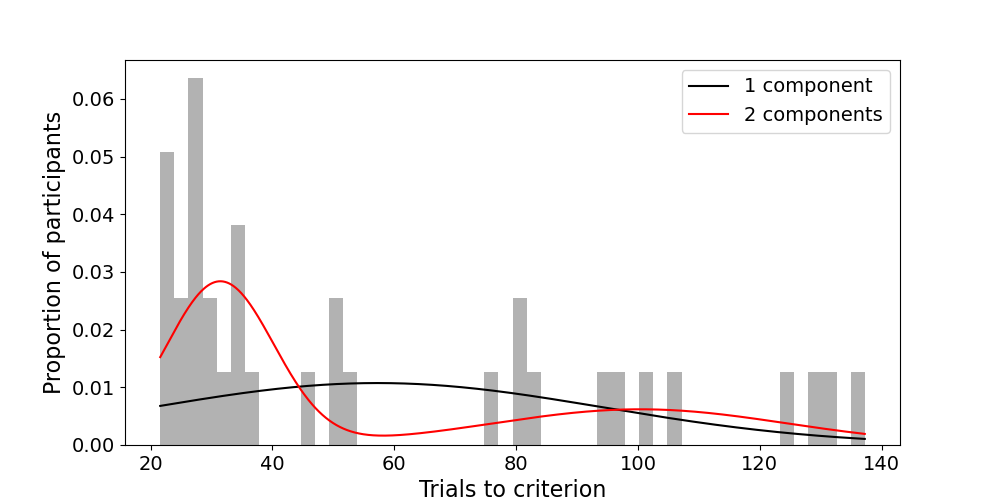
\includegraphics[width=.8\textwidth]{../figures/fig_exp_2_gmm.png}
%DIFDELCMD <   %%%
\DIFdelendFL \DIFaddbeginFL 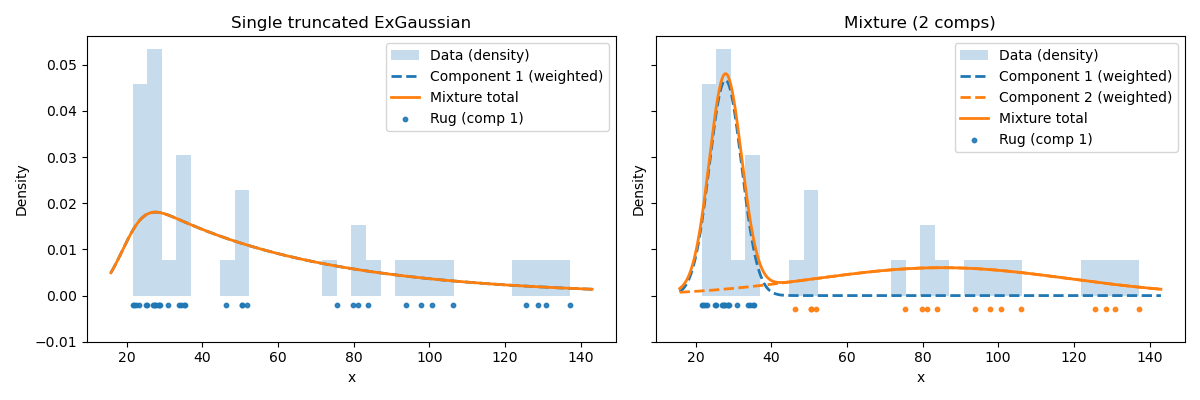
\includegraphics[width=1\textwidth]{../figures/fig_exp_2_mm_trunc_exgauss_compare.png}
  \DIFaddendFL \caption{
      Relative frequency histogram of the
      trials-to-criterion \DIFdelbeginFL \DIFdelFL{observed }\DIFdelendFL \DIFaddbeginFL \DIFaddFL{collapsed }\DIFaddendFL across all \DIFdelbeginFL \DIFdelFL{three
      }\DIFdelendFL \DIFaddbeginFL \DIFaddFL{participants
      and }\DIFaddendFL conditions in Experiment \DIFdelbeginFL \DIFdelFL{3. }\DIFdelendFL \DIFaddbeginFL \DIFaddFL{2. }\DIFaddendFL The \DIFdelbeginFL \DIFdelFL{black line represents
      }\DIFdelendFL \DIFaddbeginFL \DIFaddFL{left panel shows
      }\DIFaddendFL the best \DIFdelbeginFL \DIFdelFL{fit of the }\DIFdelendFL \DIFaddbeginFL \DIFaddFL{fitting }\DIFaddendFL one-component \DIFdelbeginFL \DIFdelFL{Gaussian Mixture
      Model}\DIFdelendFL \DIFaddbeginFL \DIFaddFL{ExGaussian
      distribution}\DIFaddendFL , and the \DIFdelbeginFL \DIFdelFL{red line represents }\DIFdelendFL \DIFaddbeginFL \DIFaddFL{right panel shows }\DIFaddendFL the \DIFdelbeginFL \DIFdelFL{best fit }\DIFdelendFL \DIFaddbeginFL \DIFaddFL{two
      components }\DIFaddendFL of the \DIFdelbeginFL \DIFdelFL{two-component Gaussian Mixture Model}\DIFdelendFL \DIFaddbeginFL \DIFaddFL{best-fitting two component
      ExGaussian mixture model}\DIFaddendFL .
}
  \DIFdelbeginFL %DIFDELCMD < \label{fig_gmm_hist_2}
%DIFDELCMD < %%%
\DIFdelendFL \DIFaddbeginFL \label{fig_mm_hist_2}
\DIFaddendFL \end{figure}

%DIF <  AIC for 1 component: 317.77535652645616
%DIF <  AIC for 2 components: 317.3995958509652
%DIF <  
%DIF <  BIC for 1 component: 320.8280775756885
%DIF <  BIC for 2 components: 325.03139847404606
%DIF <  
%DIF <  LRT statistic: 6.3757606754909375
%DIF <  Degrees of freedom: 3
%DIF <  P-value: 0.09469309595624516
\DIFdelbegin %DIFDELCMD < 

%DIFDELCMD < %%%
\DIFdelend Figure \ref{fig_exp_2_t2c}A shows the mean
trials-to-criterion in each condition of Experiment \DIFdelbegin \DIFdel{3. }\DIFdelend \DIFaddbegin \DIFadd{2. }\DIFaddend An
independent-samples t-test revealed no significant effect of
condition (\DIFdelbegin \DIFdel{$t(32.0)=0.69$, $p = .50$, $\eta^2 = .01$}\DIFdelend \DIFaddbegin \DIFadd{$t(32.0)=1.37$, $p = .18$, $d = .47$}\DIFaddend ).  The mean
number of problems solved by each participant is shown in
Figure \ref{fig_exp_2_t2c}B. An independent-samples t-test
revealed no significant effect of condition (\DIFdelbegin \DIFdel{$t(32) =
-0.49$, $p = .63$, $\eta^2 = .01$}\DIFdelend \DIFaddbegin \DIFadd{$t(32) =
-1.99$, $p = .06$, $d = -.68$}\DIFaddend ).

%DIF <    Source  ddof1  ddof2        F     p-unc       np2
%DIF <  0    cnd      1     32  0.47046  0.497715  0.014489
%DIF <  
%DIF <         A          B         T   dof     p-unc
%DIF <  0  delay  immediate  0.685901  32.0  0.497715
\DIFdelbegin %DIFDELCMD < 

%DIFDELCMD < %%%
%DIF <    Source  ddof1  ddof2         F    p-unc       np2
%DIF <  0    cnd      1     32  0.235294  0.63093  0.007299
%DIF <  
%DIF <         A          B         T   dof    p-unc
%DIF <  0  delay  immediate -0.485071  32.0  0.63093
%DIFDELCMD < 

%DIFDELCMD < %%%
\DIFdelend \begin{figure}
  \centering
  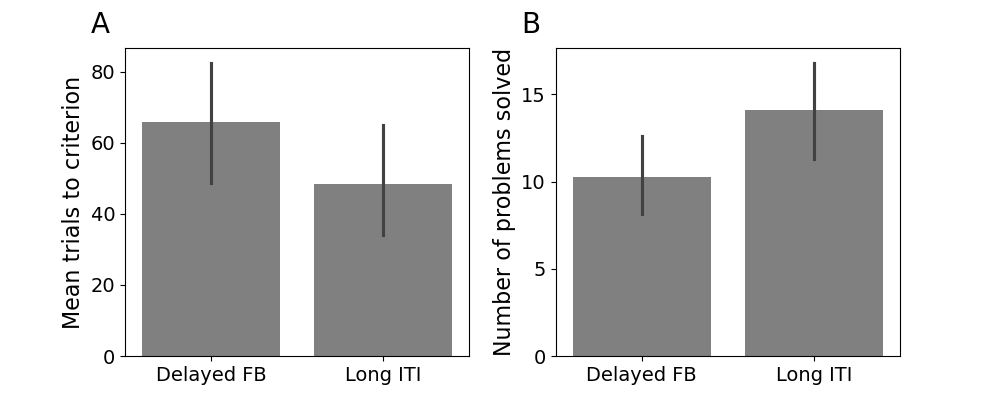
\includegraphics[width=.8\textwidth]{../figures/fig_exp_2_t2c.png}
    \caption{
        \textbf{A}: Mean trials to criterion in each
        condition of Experiment \DIFdelbeginFL \DIFdelFL{3. }\DIFdelendFL \DIFaddbeginFL \DIFaddFL{2. }\DIFaddendFL Error bars are standard
        errors of the mean.
        %
        \textbf{B}: Mean number of problems solved in each
        condition of Experiment \DIFdelbeginFL \DIFdelFL{3. }\DIFdelendFL \DIFaddbeginFL \DIFaddFL{2. }\DIFaddendFL Error bars are standard
        errors of the mean.
}
  \label{fig_exp_2_t2c}
\end{figure}

\DIFdelbegin %DIFDELCMD < \subsection{Discussion of Experiments 2 and 3}
%DIFDELCMD < %%%
\DIFdel{Experiment 2 clearly }\DIFdelend \DIFaddbegin \subsection{Discussion of Experiments 1 and 2}
\DIFadd{Experiment 1 }\DIFaddend showed that a short feedback delay of \DIFaddbegin \DIFadd{only }\DIFaddend 3.5
s slowed criterial learning. In contrast, increasing the ITI
\DIFdelbegin \DIFdel{to this same value }\DIFdelend \DIFaddbegin \DIFadd{from 500 ms to 3.5 s }\DIFaddend had no effect on learning. The task we
used was one-dimensional category learning, but we isolated
criterial learning by instructing participants about the
optimal strategy. Specifically, we told them which stimulus
dimension was relevant and that there was no trial-by-trial
variability on the irrelevant dimension. Although these
results strongly suggest that the feedback delay had its
interfering effects on criterial learning, Experiment \DIFdelbegin \DIFdel{3 }\DIFdelend \DIFaddbegin \DIFadd{2 }\DIFaddend was
designed to \DIFdelbegin \DIFdel{confirm }\DIFdelend \DIFaddbegin \DIFadd{complement }\DIFaddend this inference. The goal here was to
examine the effects of the same feedback delays and ITIs on
performance in a one-dimensional category-learning task that
did not require any criterial learning, but did require
category-learning processes that are thought to mediate rule
discovery (e.g., rule selection and switching). If the
feedback delay effects observed in Experiment \DIFdelbegin \DIFdel{2 }\DIFdelend \DIFaddbegin \DIFadd{1 }\DIFaddend were acting
on some general category-learning skill then we should have
seen the same interfering effects of feedback delay in
Experiment \DIFdelbegin \DIFdel{3. }\DIFdelend \DIFaddbegin \DIFadd{2. }\DIFaddend However, if the feedback-delay interference of
Experiment \DIFdelbegin \DIFdel{2 }\DIFdelend \DIFaddbegin \DIFadd{1 }\DIFaddend was operating selectively on criterial
learning, then it should disappear in Experiment \DIFdelbegin \DIFdel{3}\DIFdelend \DIFaddbegin \DIFadd{2}\DIFaddend , since no
criterial learning was required.  Our results strongly
supported this latter prediction.  Therefore, Experiments \DIFdelbegin \DIFdel{2 and 3 }\DIFdelend \DIFaddbegin \DIFadd{1
and 2 }\DIFaddend together strongly suggest that criterial learning is
impaired by feedback delays and is relatively unaffected by
the length of the ITI.

\DIFdelbegin \DIFdel{Two prior studies investigated similar issues. First, Ell
and colleagues reported that feedback delay and also a concurrent memory-scanning task each impaired }\DIFdelend \DIFaddbegin \DIFadd{Whereas the results of Experiment 1 seem clear, the
Experiment 2 results are weaker since they suggest a null
result. Although it impossible to rule out the possibility
that Experiment 2 missed some small effect of feedback delay
due to insufficient power, the null results found there are
consistent with a wide variety of other evidence. In
particular, a variety of other studies have reported that
feedback delays of up to 10 s do not significantly slow
one-dimensional }\DIFaddend rule-based \DIFdelbegin \DIFdel{category learning \mbox{%DIFAUXCMD
\parencite{ell2009critrial}}\hskip0pt%DIFAUXCMD
. Based on
these results, they hypothesized that criterial learning may
be tied to working-memory capacity and therefore to explicit
cognitive mechanisms. However, }\DIFdelend \DIFaddbegin \DIFadd{learning \mbox{%DIFAUXCMD
\parencite{DunnEtAl2012,
    ell2009critrial, MaddoxAshbyBohil2003, MaddoxIng2005,
Worthyetal2013}}\hskip0pt%DIFAUXCMD
. In addition, many studies have reported
evidence that one-dimensional rule-based learning recruits
working memory and executive attention, but not procedural
learning \mbox{%DIFAUXCMD
\parencite[for reviews, see,
e.g.,][]{AshbySmithRosedahl2020, AshbyValentin2017}}\hskip0pt%DIFAUXCMD
. So the
results of Experiment 2 are consistent with all of these
studies. On the other hand, several of these feedback-delay
studies did not use binary-valued stimulus dimensions, so
some }\DIFaddend criterial learning was \DIFdelbegin \DIFdel{confounded with rule selection and task difficulty in their
design. Furthermore, \mbox{%DIFAUXCMD
\textcite{ell2009critrial} }\hskip0pt%DIFAUXCMD
found that
feedbackdelay only impaired learning when working memory
demand was high -- that is, when participants had to learn
more than one response criterion for optimal performance. In
contrast, we found that feedback delay impairs learning even
when working memory demands are trivial (participants never
have to keep in mind more than one criterion)}\DIFdelend \DIFaddbegin \DIFadd{required. If so, then why did
they all report no effect of feedback delay? It is important
to note that criterial learning was not the focus of any of
these studies, and as a result, in all of these previous
studies the optimal criterion was always set exactly midway
between the category prototypes, which makes criterial
learning trivial. For example, under these conditions,
criterial learning might not even require feedback. The
unsupervised category-learning experiments reported by
\mbox{%DIFAUXCMD
\textcite{ashby1999dominance} }\hskip0pt%DIFAUXCMD
provide strong support for
this because all of their rule-based participants learned
the correct criterion (which was midway between the category
means), even though the task was completely unsupervised.
}

\DIFadd{We know of only one previous study that reported impaired
one-dimensional rule-based category learning when feedback
was delayed \mbox{%DIFAUXCMD
\parencite{ell2009critrial}}\hskip0pt%DIFAUXCMD
. However, in this
study, a feedback delay only impaired performance in a
condition with four contrasting categories that required
learning three different response criteria. So this task was
considerably more complex than any of the other
feedback-delay studies, which all used two contrasting
categories that required the learning of only one response
criterion}\DIFaddend . 

\DIFdelbegin \DIFdel{Second}\DIFdelend \DIFaddbegin \DIFadd{One other study with similar goals to ours studied how
manipulations of category base rates affect criterial
learning in one-dimensional rule-based categorization.
Specifically}\DIFaddend , \textcite{bohil2014implicit} reported that
\DIFdelbegin \DIFdel{the
effects of unequal base rates on }\DIFdelend \DIFaddbegin \DIFadd{changes in }\DIFaddend criterion placement in \DIFdelbegin \DIFdel{rule-based category learning were diminished under delayed
feedback and also under an observational trainingprotocol
that is also thought to selectively impair basal
ganglia-dependent associative-learning mechanisms}\DIFdelend \DIFaddbegin \DIFadd{response to changes in
base rate were diminished when feedback was delayed (and
also by observational training)}\DIFaddend . These results are
consistent with our findings. However, because they were
obtained by manipulating base rates, it is difficult to
conclude that the delay affected criterial learning,
\emph{per se}. For example, consider a simple two-stage
model in which the first stage learns the base rates and the
second stage uses what the first stage learned to adjust the
response criterion appropriately. The
\textcite{bohil2014implicit} results are also consistent
with the hypothesis that the feedback delay impaired the
first of these stages but not the second. Our results
strongly suggest that feedback delays impair criterial
learning (and therefore the second of these hypothetical
stages).

\DIFdelbegin %DIFDELCMD < \section{General Discussion}
%DIFDELCMD < %%%
\DIFdel{We developed three novel models of criterial learning that
were designed to explore how feedback delay and
ITI duration
affect criterial learning . Two of these models assumed that decisions are made }\DIFdelend \DIFaddbegin \section{New Computational Models of Criterial Learning}
\DIFadd{The results of Experiments 1 and 2 seem to suggest that
criterial learning is a form of procedural learning, which
previous research suggests is of SR associations
\mbox{%DIFAUXCMD
\parencite{AshbyWaldron1999, CasaleEtAl2012}}\hskip0pt%DIFAUXCMD
. If so, then
the criterion is simply the sensory, perceptual, or
cognitive value that separates representations associated
with contrasting responses. However, before accepting this
conclusion, it is important to ask whether our results might
also be compatible with an account in which the criterion is
held is some form of working or short-term memory and
updated trial by trial. 
}

\DIFadd{To address this question, we developed computational models
of criterial learning within two broad architectures and
examined their sensitivity to ITI duration and feedback
delay. The architectures differed in whether they assume
that the response criterion is explicitly represented in
memory. In the first architecture, the criterion is stored
in memory, and responses are generated }\DIFaddend by comparing the
current percept \DIFdelbegin \DIFdel{to a
stored referent, or criterion , and that the remembered value
of this criterion is updated following error feedback via a
gradient-descent learning rule.  The first }\DIFdelend \DIFaddbegin \DIFadd{with this stored referent. The criterion is
updated after error feedback using a gradient-descent rule.
Models in this class can exhibit sensitivity to ITI and
feedback delay in three distinct ways: (1) perceptual drift,
where stimulus representations change over time, (2)
criterial drift, where the stored criterion shifts over
time, and (3) updating that is sensitive to feedback delays,
where the magnitude of criterion updates decreases with
longer feedback delays. In the second architecture, no
explicit criterion is stored. Instead, reinforcement
learning forms direct stimulus--response associations that
drive performance.  Sensitivity to ITI and feedback delay
arise from perceptual drift and/or delay-sensitive updating,
but criterial drift is not possible since no criterion is
represented.
}

\DIFadd{For each }\DIFaddend of these models, \DIFdelbegin \DIFdel{the time-dependent drift model, posits that both the criterion and the percept }\DIFdelend \DIFaddbegin \DIFadd{denote the time of stimulus
presentation on the current trial by T$_\text{S}$, the
response time by T$_\text{R}$, the time when feedback is
displayed by T$_\text{F}$, and the time when the stimulus
that begins the next trial is displayed by T$_{\text{S}^+}$.
Then note that the feedback delay equals $\text{t}_\text{FD}
= \text{T}_\text{F} - \text{T}_\text{R}$ and the duration of
the ITI equals $\text{t}_\text{ITI} = \text{T}_{\text{S}^+}
- \text{T}_\text{F}$.
}

\subsection{Models that assume a stored criterion}
\DIFadd{These models assume that the observer constructs a response
criterion, maintains it in memory, and makes
decisions by comparing the percept to this criterion. They
may further posit that both the stored criterion and the
perceived stimulus value }\DIFaddend drift over time, \DIFdelbegin \DIFdel{leading to
similar impairments when feedback is delayed or the ITI is increased. The second model, }\DIFdelend \DIFaddbegin \DIFadd{with the extent of
drift increasing both within a trial and across consecutive
trials. In addition, they may assume that the learning rate
for updating the criterion decreases as the feedback delay
increases.
}

\DIFadd{Let $x_n(t)$ and $c_n(t)$ denote the values of the percept
and the criterion, respectively, on trial $n$ at time $t$.
Then the decision rule on trial $n$ is:
}\begin{equation}
  \DIFadd{\text{Respond } R_n =
  \begin{cases}
    \text{A}, & \text{if ~} x_n(\text{T}_\text{S}) \leq c_n(\text{T}_\text{S})  \\
    \text{B}, & \text{if ~} x_n(\text{T}_\text{S}) > c_n(\text{T}_\text{S}).
  \end{cases}
  \label{eq:DR}
}\end{equation}
\DIFadd{Note that this equation indicates that the response is made
immediately upon stimulus presentation. We therefore are not
explicitly modeling the time-extended cognitive processes
that govern evidence accumulation and the corresponding
response time.
}

\DIFadd{If positive feedback is received, then the value of the
criterion remains unchanged for the next trial (except for
drift -- see equation \ref{eq:criterion}).  The rationale
here is that if the response is correct, then the observer
has effectively gained zero information about how their
criterion should be modified.  If negative feedback is
received, then the criterion is modified according to the
standard model
\mbox{%DIFAUXCMD
\parencite{SuttonBarto1998}}\hskip0pt%DIFAUXCMD
:
}\begin{equation}
\DIFadd{c_n(\text{T}_\text{F}+ \Delta_t) = c_n(\text{T}_\text{F}) + \frac{\alpha}{t_{FD}} }[\DIFadd{x_n(\text{T}_\text{F}) - c_n(\text{T}_\text{F})}]\DIFadd{,
\label{RL}
}\end{equation}
\DIFadd{where $\alpha$ is a learning-rate parameter, and $\Delta_t$
is the time it takes to complete the updating.  It is
straightforward to show that }\DIFaddend the \DIFdelbegin \DIFdel{delay-sensitive learning
model
, assumes that although neither the percept nor the criterion drift over time, optimal criterial learning
requires immediate feedback }\DIFdelend \DIFaddbegin \DIFadd{iterative equation \ref{RL}
is equivalent to computing a weighted mean (weighted by
recency) of the values of all percepts that occur on error
trials \mbox{%DIFAUXCMD
\parencite[e.g.,][]{Ashby2017}}\hskip0pt%DIFAUXCMD
. This updating rule
will gradually converge on the optimal criterion value
(i.e., the value of the criterion that maximizes accuracy).  
}

\DIFadd{The term $\alpha/t_{FD}$ captures the notion that the
magnitude of the update decreases as the feedback delay
increases}\DIFaddend .  As a result, \DIFdelbegin \DIFdel{this model
predicts that increasing the feedback delay will slow the
rate of criterial learning . The third model,
the
reinforcement-learning model , assumes }\DIFdelend \DIFaddbegin \DIFadd{when feedback is delayed, the
system becomes less responsive to errors, leading to slower
learning compared to immediate feedback conditions. However,
since this model is consistent with the idea }\DIFaddend that criterial
learning \DIFdelbegin \DIFdel{arises through the gradual formation of stimulus-response associations, rather than via the
construction of a response criterion.
This model also
assumes that the rate at which these associations are learned is slowed by feedback delays. }\DIFdelend \DIFaddbegin \DIFadd{relies on working memory -- and the available
evidence suggests that logical reasoning and working memory
are unaffected by feedback delays of several seconds
\mbox{%DIFAUXCMD
\parencite[e.g., in one-dimensional rule-based category
learning tasks;][]{ell2009critrial, MaddoxAshbyBohil2003,
MaddoxIng2005} }\hskip0pt%DIFAUXCMD
-- the learning process described in equation
\ref{RL} likewise may be unaffected by feedback delay. We
therefore also investigated a version of the model in which
the term $\alpha/t_{FD}$ is replaced by $\alpha$, making the
learning rate independent of feedback delay.
}

\DIFadd{This model further assumes that both the stimulus and the
criterion representations may drift randomly throughout the
duration of time they are maintained in working memory. The
representation of the criterion must always be maintained in
working memory, whereas drift in the stimulus representation
affects performance up until the feedback is presented, but
not afterwards (i.e., because the equation \ref{RL} updating
rule depends on the value of the current stimulus
representation). We modeled the drift in both the criterion
and the percept by adding white noise to their initial
values. Specifically, we assumed that for all
$t>\text{T}_\text{S}$
}\begin{equation}
  \DIFadd{c_n(t) = c_n(\text{T}_\text{S}) + \eta_c \epsilon(t),
  \label{eq:criterion}
}\end{equation}
\DIFadd{and
}\begin{equation}
  \DIFadd{x_n(t) = x_n(\text{T}_\text{S}) + \eta_x \epsilon(t),
  \label{eq:percept}
}\end{equation}
\DIFadd{where $\epsilon(t)$ is white noise and $\eta_c$ and $\eta_x$
are parameters that determine the amount of drift over time.
Note that these parameters are permitted to be equal to
zero, which is equivalent to assuming that the criterion
and/or the percept do not drift over time at all.
}\DIFaddend 

\DIFdelbegin \DIFdel{Simulations of these models in a task that was structurally
identical to Experiment 2 revealed that the time-dependent
drift model typically predicts that the most important
variable for criterial learning is the total amount of time
}\DIFdelend \DIFaddbegin \DIFadd{This model predicts that }\DIFaddend between the \DIFdelbegin \DIFdel{response and
the stimulus presentation that
defines the next trial. Where the feedback is presented
within this interval is relatively unimportant. In contrast, both the delay-sensitive learning model and }\DIFdelend \DIFaddbegin \DIFadd{time of stimulus
presentation and feedback, the response criterion will drift
randomly. The amount of drift during this time will be
normally distributed with mean zero and variance
$\text{t}_\text{FD} \eta_c^2$. Similarly, the amount of
criterial drift after the updating that follows feedback and
the presentation of the stimulus on the next trial will also
be normally distributed with mean zero, but now with
variance $(\text{t}_\text{ITI}) \eta_c^2$. Predictions for
the percept are similar. Specifically, }\DIFaddend the \DIFdelbegin \DIFdel{reinforcement-learning model consistently predict that
feedback delays should impair performance more than a long
ITI}\DIFdelend \DIFaddbegin \DIFadd{amount of drift
between stimulus presentation and feedback will be normally
distributed with mean zero and variance $\text{t}_\text{FD}
\eta_x^2$}\DIFaddend .

\DIFdelbegin \DIFdel{The experiments were designed to test these predictions. Our
results strongly suggested that human criterial learning is sensitive to feedback delay but not to the
ITI duration. This suggests that }\DIFdelend \DIFaddbegin \subsection{Models that assume no criterion}
\DIFadd{A qualitatively different class of models, based on an
actor-critic architecture \mbox{%DIFAUXCMD
\parencite{SuttonBarto1998}}\hskip0pt%DIFAUXCMD
,
assume that learning is a process of associating each
stimulus with a response via reinforcement learning. These
models do not include an explicit representation of the
response criterion. Rather the criterion is simply the
mental representation that separates percepts associated
with contrasting responses. 
}

\DIFadd{In this class of models, the perceptual representation of
each stimulus is modeled as a pattern of activation across
25 sensory units that are each characterized by an
overlapping tuning curve. Each unit is maximally excited by
one specific stimulus, which we call the unit's preferred
stimulus. Specifically, the activation of the $i^\text{th}$
sensory unit on trial $n$ at time $t$ is given by
}\begin{equation}
  \DIFadd{A_i(n,t) = \text{exp} \left( \frac{-\left[d_{i,S_n(t)}\right]^2}{\sigma^2} \right)
  \label{eq:DSL_activation}
}\end{equation}
\DIFadd{where $d_{i,S_n(t)}$ is the (Euclidean) distance between the
preferred stimulus value of the $i^\text{th}$ sensory unit
and the value of the stimulus that was presented on trial
$n$ at time $t$, and $\sigma$ is a constant that increases
with perceptual noise.
}

\DIFadd{Because this class of models does not store an explicit
response criterion, it cannot incorporate criterial drift.
It can, however, incorporate perceptual drift. In this case,
the value of }\DIFaddend the \DIFdelbegin \DIFdel{delay-sensitive learning model and the reinforcement-learning model provide a better account of human behavior across wide ranges of their respective
parameter spaces than the time-dependent drift model}\DIFdelend \DIFaddbegin \DIFadd{current stimulus used to compute sensory
unit activation (Equation~\ref{eq:DSL_activation}) is
assumed to drift over time according to
}\begin{equation}
  \DIFadd{S_n(t) = S_n(\text{T}_\text{S}) + \eta_S \epsilon(t),
  \label{eq:stimulus_drift_RL}
}\end{equation}
\DIFadd{where $\eta_S$ scales the magnitude of the drift and
$\epsilon(t)$ is a noise process}\DIFaddend .

The \DIFdelbegin \DIFdel{time-dependent drift model was based on the idea that criterial learning
might be entirely supported by working
memory. The assumption of drift in this model stems from the understanding that maintaining items in working memory is inherently challenging. The longer an item is held, the
more likely it is
to deteriorate. Therefore, the model
predicts that performance should deteriorate as the
time
between the response on }\DIFdelend \DIFaddbegin \DIFadd{model includes two decision or actor units -- one
associated with each of the two possible responses.
Initially, each sensory unit is connected to both actor
units with some random connection strength. Let
$\omega_{iJ}(n)$ denote the strength of the connection
between sensory unit $i$ and actor unit $J$ (for $J$ = A or
B) on }\DIFaddend trial $n$\DIFdelbegin \DIFdel{and stimulus presentation
on trial $n+1$ increases, regardless of how this interval is divided between feedback delay}\DIFdelend \DIFaddbegin \DIFadd{. Then the activation in actor unit $J$ on
trial $n$ at time $t$, denoted by $V_J(n,t)$, equals
}\begin{equation}
  \DIFadd{V_J(n,t) = \sum_{i} \omega_{iJ}(n) A_i(n,t).
}\end{equation}
\DIFadd{A response is selected by comparing the activations in
competing actor units immediately after stimulus
presentation, that is, at time $t=\text{T}_\text{S}$,  using
the following the decision rule:
}\begin{equation}
 \DIFadd{\text{Respond } R_n =
  \begin{cases}
    A, & \text{if $V_A(n,\text{T}_\text{S}) > V_B(n,\text{T}_\text{S})$}\\
    B, & \text{if $V_A(n,\text{T}_\text{S}) \leq V_B(n,\text{T}_\text{S}).$}
  \end{cases}
}\end{equation}

\DIFadd{The connection strengths $\omega_{iA}(n)$ }\DIFaddend and
\DIFdelbegin \DIFdel{ITI. The results of Experiments 1 and 2 strongly disconfirm this prediction.
}%DIFDELCMD < 

%DIFDELCMD < %%%
\DIFdel{In contrast, the delay-sensitive learning model was inspired
by the
idea that a response criterion might be encoded in a
more stable memory system.
One appealing candidate for this
function is
the cerebellum, }\DIFdelend \DIFaddbegin \DIFadd{$\omega_{iB}(n)$ are updated after feedback is received on
each trial according to standard reinforcement learning
rules \mbox{%DIFAUXCMD
\parencite{SuttonBarto1998}}\hskip0pt%DIFAUXCMD
. If the feedback is
positive, then for J = A or B:
}\begin{equation}
  \DIFadd{\omega_{i\text{J}}(n) = \omega_{i\text{J}}(n-1) + \frac{\alpha_{actor}}{t_\text{FD}} A_i(n,\text{T}_\text{F}) V_\text{J}(n,\text{T}_\text{F}) \delta(n-1) }[\DIFadd{1-\omega_{i\text{J}}(n-1)}]\DIFadd{,
  \label{eq:W+}
}\end{equation}
\DIFaddend where \DIFdelbegin \DIFdel{synaptic plasticity has
been shown to follow a gradient descent learning rule and also to be sensitive to feedback timing
\mbox{%DIFAUXCMD
\parencite{brudner2016delayed, held_adaptation_1966,
honda_adaptation_2012, kitazawa_effects_1995,
kitazawa_prism_2002}}\hskip0pt%DIFAUXCMD
. Finally, }\DIFdelend \DIFaddbegin \DIFadd{$\alpha_{actor}$ is the learning-rate of }\DIFaddend the \DIFdelbegin \DIFdel{reinforcement-learning
model draws on the idea that criterial learning could emerge
through }\DIFdelend \DIFaddbegin \DIFadd{actor,
and $\delta(n-1)$ is the reward prediction error on trial
$n-1$. The last term prevents the weight from exceeding 1.
Note that the increase in synaptic strength is scaled by the
product of the pre- and postsynaptic activation values. Also
note that, as in equation~\ref{RL}, the learning rate is
scaled by the inverse of the feedback delay. If the feedback
is negative, then 
}\begin{equation}
  \DIFadd{\omega_{i\text{J}}(n) = \omega_{i\text{J}}(n-1) + \frac{\alpha_{actor}}{t_\text{FD}} A_i(n,\text{T}_\text{F}) V_\text{J}(n,\text{T}_\text{F}) \delta(n-1) \omega_{i\text{J}}(n-1).
  \label{eq:W-}
}\end{equation}
\DIFadd{Now the last term prevents the weight from falling below 0.
Note that on error trials, $\delta(n-1)$ will be negative,
so equation \ref{eq:W-} decreases the synaptic weight.
}

\DIFadd{The reward prediction error on trial $n-1$ is defined as the
value of the obtained reward, denoted by $R(n-1)$ minus the
value of the predicted reward, denoted by $P(n-1)$:
}\begin{equation}
  \DIFadd{\delta(n-1) = R(n-1) - P(n-1).
}\end{equation}
\DIFadd{The predicted reward on trial $n$ is determined by the
critic via
}\begin{equation}
  \DIFadd{P(n) = P(n-1) + \frac{\alpha_{critic}}{t_\text{FD}} \delta(n-1),
  \label{eq:Pcritic}
}\end{equation}
\DIFadd{where $\alpha_{critic}$ is the learning rate of the critic.
Note that this learning rate is again scaled by the inverse
of the feedback delay. 
}

\DIFadd{Much evidence suggests that this type of }\DIFaddend stimulus-response
\DIFdelbegin \DIFdel{association learning driven by
dopamine-dependent synaptic plasticity in the striatum. This
process aligns with established theories of category
learning that posit a key role to this learning process in the basal ganglia \mbox{%DIFAUXCMD
\cite{AshbyCOVIS1998}}\hskip0pt%DIFAUXCMD
.   }\DIFdelend \DIFaddbegin \DIFadd{learning is mediated largely within the striatum, and is
facilitated by a dopamine-mediated reinforcement learning
signal that is time dependent
\mbox{%DIFAUXCMD
\parencite[e.g.,][]{ValentinMaddoxAshby2014}}\hskip0pt%DIFAUXCMD
. Specifically,
the dopamine signal generated by positive feedback appears
to peak at around 500 ms after feedback and then decay back
to baseline levels within 2 or 3 s
\mbox{%DIFAUXCMD
\parencite{YagishitaEtAl2014}}\hskip0pt%DIFAUXCMD
. As a result, synaptic
plasticity at cortical-striatal synapses is attenuated with
increasing feedback delays \mbox{%DIFAUXCMD
\parencite{YagishitaEtAl2014}}\hskip0pt%DIFAUXCMD
.
The scaling of $\alpha_{actor}$ and $\alpha_{critic}$ by
$1/{t_\text{FD}}$ is one way to model this phenomenon.
However, it is possible that stimulus-response association
learning is mediated by other brain systems that are less
sensitive to feedback delay. For this reason, we also
investigated a version of the model in which the updating
equations are independent of feedback delay. In this
version, the term $\alpha_{actor}/t_\text{FD}$ is replaced
by $\alpha_{actor}$ in equations \ref{eq:W+} and \ref{eq:W-}
and the term $\alpha_{critic}/t_\text{FD}$ is replaced by
$\alpha_{critic}$ in equation \ref{eq:Pcritic}.
}\DIFaddend 

\DIFdelbegin \DIFdel{Our results do not strongly favor the delay-sensitive
learning model over the reinforcement learning model or vice
versa. The critical disagreement between these accounts is whether the criterion has any real psychological meaning. In
the
delay-sensitive learning model it does }\DIFdelend \DIFaddbegin \subsection{Simulation Results}
\DIFadd{We investigated how changing the duration of the feedback
delay and the ITI affect criterial learning for each class
of model. More specifically, we simulated performance of
each model in each of the three conditions of the Experiment
1 categorization task. Each simulation continued for 200
trials or until the model responded correctly for 12 trials
in a row. For each set of parameter values, we simulated the
model 100 times and averaged the results, yielding one
observed performance metric measured in mean
trials-to-criterion for each condition. 
}

\DIFadd{Our approach was to generate predictions for each of the
three experimental conditions across a wide range of
parameter values. We then used parameter-space partitioning
(PSP) to evaluate the performance of each model
\mbox{%DIFAUXCMD
\parencite{pitt2006global}}\hskip0pt%DIFAUXCMD
. Traditional computational
modeling identifies parameter values that allow the model to
provide the best possible fit to the observed data. This
traditional approach therefore treats the single observed
data set being fit as a gold standard. Our goal instead was
to investigate the range of possible predictions of each
model. We were interested in questions such as: can a model
predict any possible outcome or is it constrained to always
predict, for example, that feedback delays impair learning?
PSP was designed to answer such questions.
}

\DIFadd{Classical PSP is defined for non-stochastic models and is
often implemented by exploring the parameter space via a
Markov chain Monte Carlo algorithm. In contrast, we used
brute force search over a grid of plausible parameter
values. Because our models are stochastic, at each sampled
set of parameter values we generated multiple simulations
and classified the results into one of a small set of
qualitative outcome patterns. PSP calculates the proportion
of the parameter space where the model makes specific
predetermined qualitative predictions. We focused on the
following four such predictions. 1) Delay impaired:
Performance is worst in the Feedback-Delay condition. 2)
Long ITI impaired: Performance is worst in the Long-ITI
condition. 3) Short ITI impaired: Performance is worst in
the Control condition. 4) Other: Two or more conditions are
tied for worst performance. For each model, the PSP analysis
quantified the proportions of the explored parameter space
where the model made each of these qualitative predictions.
}

\subsubsection{Models that assume a stored criterion}
\DIFadd{We investigated predictions of these models across a wide
range of values for the parameters $\eta_{x}$}\DIFaddend , \DIFdelbegin \DIFdel{and thus this model is psychologically similar to the time-dependent drift
model -- the main disagreement being about whether the
representation }\DIFdelend \DIFaddbegin \DIFadd{$\eta_{c}$,
and $\alpha$.  Specifically, in the case of $\alpha$,  we
stepped through every value in the interval $[0, .2]$, with
a step size of .01.  In the case of both $\eta_{x}$, and
$\eta_{c}$, we searched over the interval $[0, 5]$, with a
step size of $.1$.  We also explored the binary case of
whether or not the update rate $\alpha$ was scaled by the
feedback delay. 
}

\DIFadd{Figure~\ref{fig:criterion_results} shows the results. Panel
A lists the proportions of parameter space over which the
version of the model that is sensitive to feedback delay
predicts each of the four qualitatively different outcomes.
Note that this model predicts that the poorest performance
will be in the Feedback Delay condition for all values of
its parameters. At first glance, this result seems
surprising because it means that there are no parameter
values that make the model more sensitive to ITI than to
feedback delay. This makes sense though because increasing
the ITI has no effect on the mean criterion value -- the
only effect is to increase the criterion value's variance.
In contrast, increasing the feedback delay affects the mean
criterion value because it slows the criterion updating
process from converging on the optimal value. 
}

\begin{figure} 
  \centering
  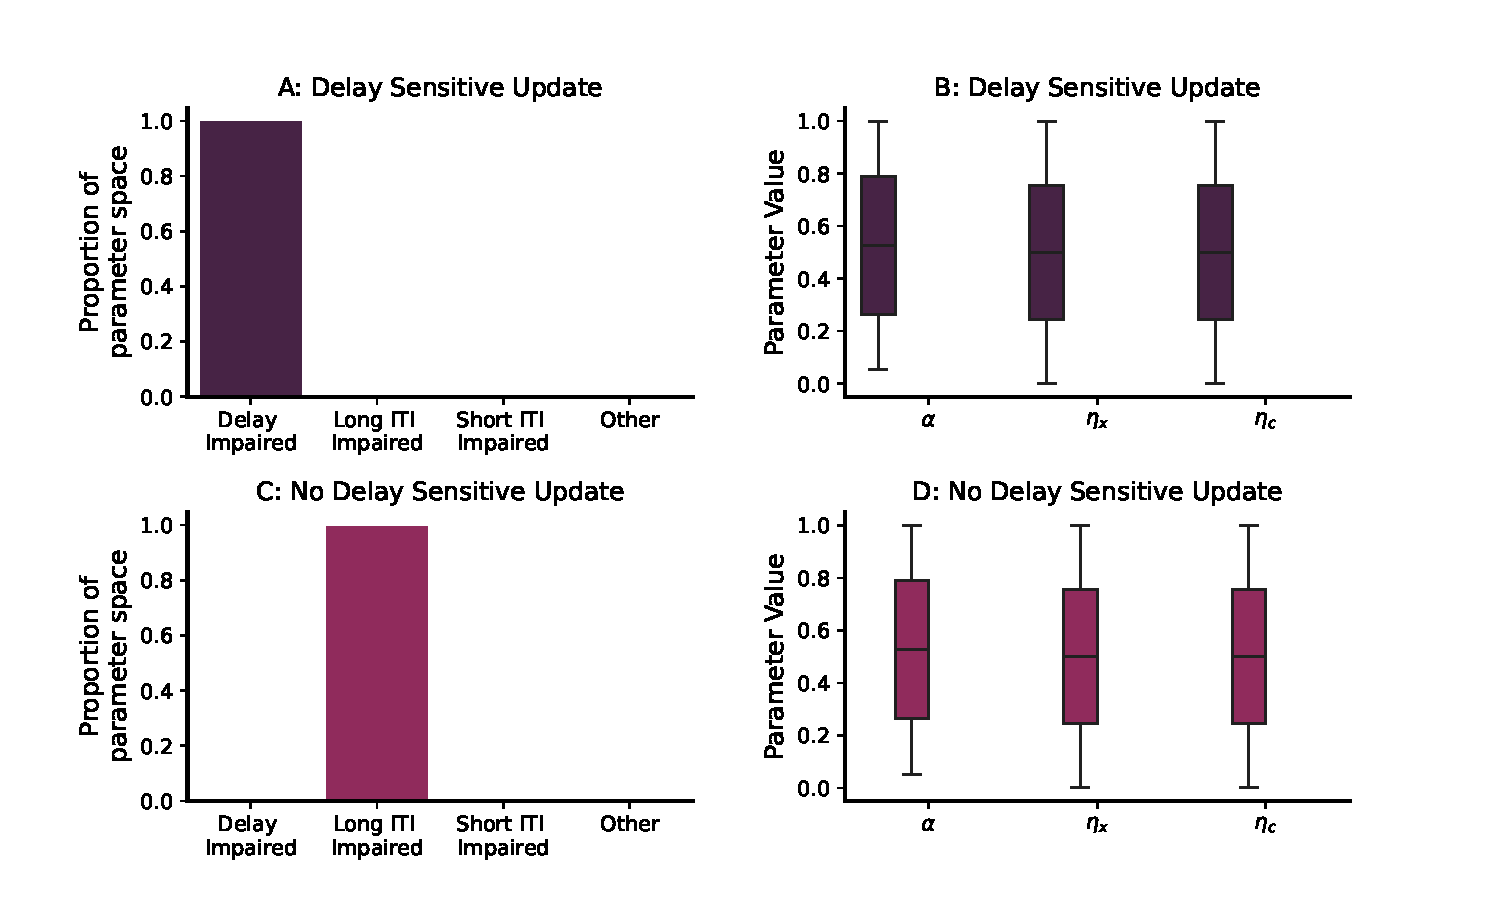
\includegraphics[width=1\textwidth]{../figures/model_new_class_II_yes_stored_criterion.pdf}
  \caption{\DIFaddFL{Simulation results for models that assume a stored criterion.  
      }\textbf{\DIFaddFL{A:}} \DIFaddFL{The proportions of parameter space where
      each of the four qualitative outcomes is predicted by
      the versions of the model that assume criterion
      updating is sensitive to feedback delay. 
      }\textbf{\DIFaddFL{B:}} \DIFaddFL{Boxplot showing the parameter ranges that
      produced the panel A results. All parameter values
      were normalized by the largest value in the search
      range, so the ordinate ranges from zero to one for all
      parameters.
      %DIF >  
      }\textbf{\DIFaddFL{C:}} \DIFaddFL{The proportions of parameter space where
      the models that assume criterion updating is
      insensitive to feedback delay predict each of the four
      qualitative outcomes. 
      }\textbf{\DIFaddFL{D:}} \DIFaddFL{Boxplot showing the parameter ranges that
      produced the panel C results.     
      %DIF > 
      }\textit{\DIFaddFL{Note:}} \DIFaddFL{In all panels, color indicates the PSP
      pattern.
}}
    \label{fig:criterion_results}
\end{figure}

\DIFadd{Panel C of Figure \ref{fig:criterion_results} shows the same
results as in panel A, except for the version of the model
in which the criterion updating process is insensitive to
feedback delay. Note that this version of the model predicts
that performance must be worst in the Long-ITI condition --
again for all values of its parameters. This result also
shows that no amount of perceptual or criterial drift allows
this version of the model to account for the Experiment 1
results. 
}

\subsubsection{Models that assume no criterion}
\DIFadd{We investigated predictions of the SR-learning model by
varying four parameters; namely, the perceptual-noise
variance $\sigma^2$, the stimulus drift parameter $\eta_S$,
and the actor and critic learning rates (i.e.,
$\alpha_{actor}$ and $\alpha_{critic}$, respectively). In
the case of $\sigma$, we searched over the interval $[1,
10]$, with a step size of $3$. For $\eta_S$, we searched
over the interval $[0, 1]$, with a step size of $.1$. For
both $\alpha_{actor}$ and $\alpha_{critic}$, we stepped
through every value in the interval $[0, .2]$, with a step
size of $.02$. We constrained our search over these
parameters to this interval because reinforcement-learning
models are prone to instability at very high learning rates
\mbox{%DIFAUXCMD
\parencite{SuttonBarto1998}}\hskip0pt%DIFAUXCMD
. As evidence of this, at higher
learning rates, the model failed to learn with any
consistency -- that is, in most cases, it failed to reach
the learning criterion (12 correct responses in a row)
within the allowable 200 trials.   We also explored the
binary case of whether or not the update rates
$\alpha_{actor}$ and $\alpha_{critic}$ were scaled by the
feedback delay. As with the other models, all scores were
normalized by the largest observed value.
}

\DIFadd{The results are described in Figure \ref{fig:RL_results}.
Panel A lists the proportions of parameter space over which
the feedback-delay sensitive version of the model predicts
each qualitatively different outcome. Note that across the
vast majority of its parameter space, this model predicts
that an increase in feedback delay will impair performance
more than an increase in ITI. 
}

\begin{figure} 
  \centering
  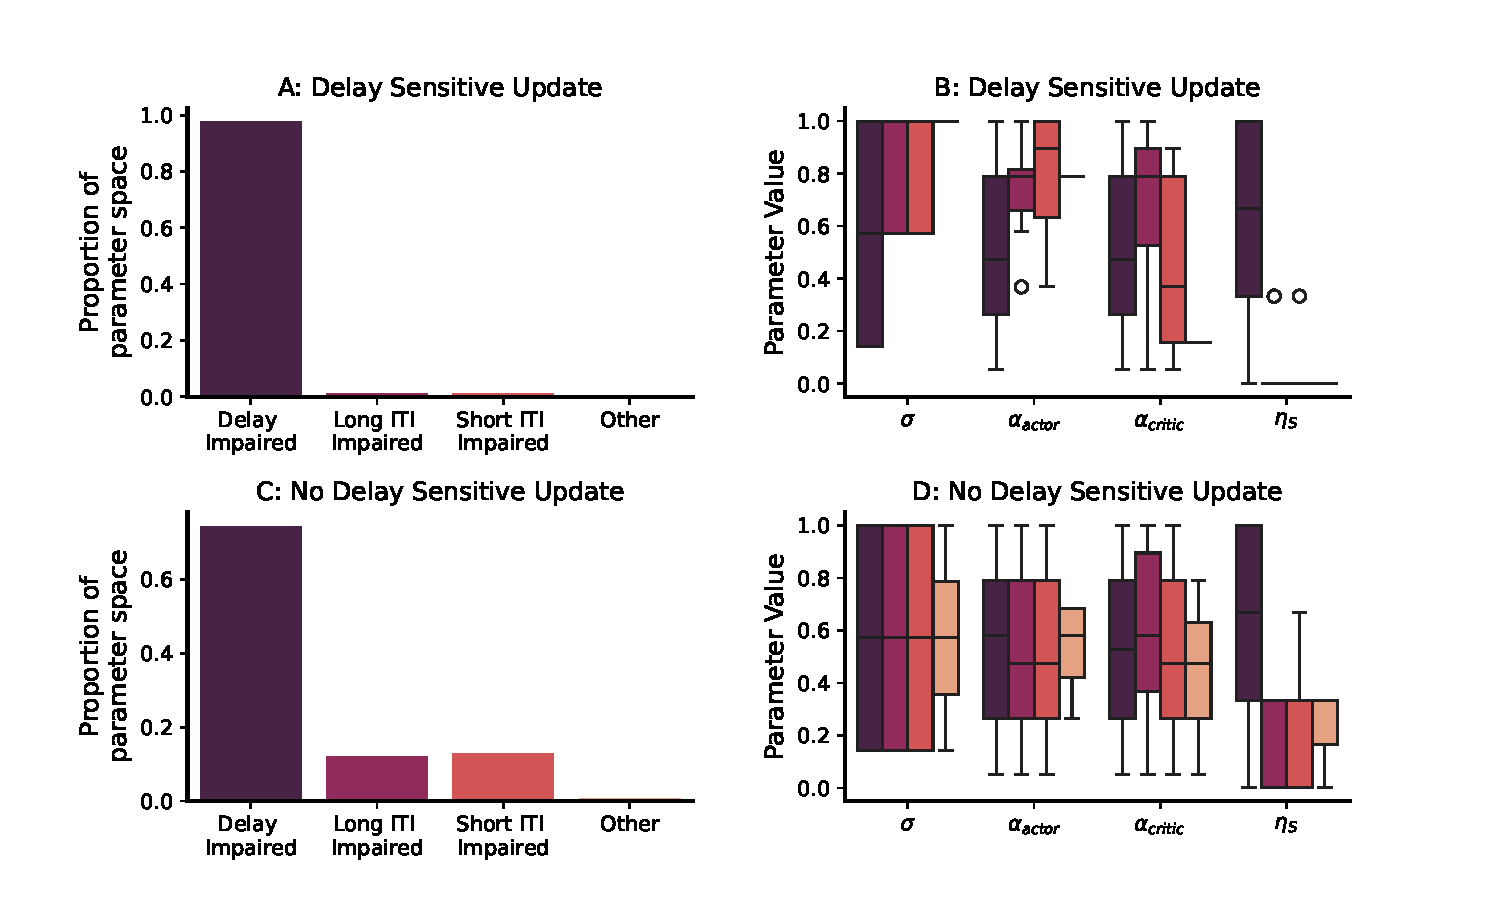
\includegraphics[width=1\textwidth]{../figures/model_new_class_I_no_stored_criterion.pdf}
  \caption{ \DIFaddFL{Simulation results for models that assumed
      stimulus-response learning and therefore no stored
      criterion.  
      }\textbf{\DIFaddFL{A:}} \DIFaddFL{The proportions of parameter space where
      each of the four qualitative outcomes is predicted by
      the versions of the model that assume synaptic
      updating is sensitive to feedback delay.
      }\textbf{\DIFaddFL{B:}} \DIFaddFL{Boxplot showing the parameter ranges that
      produced the panel A results.     All parameter values
      were normalized by the largest value in the search
      range, so the ordinate ranges from zero to one for all
      parameters.
      %DIF >  
      }\textbf{\DIFaddFL{C:}} \DIFaddFL{The proportions of parameter space where
      the models that assume synaptic updating is
      insensitive to feedback delay predict each of the four
      qualitative outcomes. 
      }\textbf{\DIFaddFL{D:}} \DIFaddFL{Boxplot showing the parameter ranges that
      produced the panel C results.     
      %DIF > 
      }\textit{\DIFaddFL{Note:}} \DIFaddFL{In all panels, color indicates the PSP
      pattern.
}}
  \label{fig:RL_results}
\end{figure}

\DIFadd{Figure \ref{fig:RL_results}C shows the proportions of
parameter space over which the models that assume synaptic
updating is insensitive to feedback delay predict each of
the four qualitative outcomes. Surprisingly, this version of
the model also almost always predicts the poorest
performance in the Feedback-Delay condition. What is going
on here? First, note that even if
$\alpha_{actor}/t_\text{FD}$ and
$\alpha_{critic}/t_\text{FD}$ in equations \ref{eq:W+},
\ref{eq:W-}, and \ref{eq:Pcritic} are replaced by
$\alpha_{actor}$ and $\alpha_{critic}$, respectively, then
equations \ref{eq:W+} and \ref{eq:W-} are still sensitive to
feedback delay because the pre- and postsynaptic activations
in equations \ref{eq:W+} and \ref{eq:W-} are computed at the
time of feedback -- that is, at time T$_\text{F}$. So the
longer that the feedback is delayed, the more time there is
for the stimulus representation to drift from its true
value. As a result, this model predicts that delayed
feedback will impair learning, even though the amount of
updating on each trial does not depend on feedback delay.
Second, note that all versions of this model are generally
insensitive to the length of the ITI. The stored-criterion
models are adversely affected by a long ITI because the
criterion drifts during this time and large drift means that
on the next trial a decision will be made with a suboptimal
value }\DIFaddend of the criterion\DIFdelbegin \DIFdel{is stable and if the updating of the criterion is }\DIFdelend \DIFaddbegin \DIFadd{. But there is no criterion to drift
in the SR-learning models. The stimulus will continue to
drift during the ITI in these models, but with no
consequence, because after the synaptic updating that occurs
with presentation of the feedback, the stimulus
representation on the current trial is no longer needed. So
all versions of the SR-learning model are more }\DIFaddend sensitive to
feedback delay \DIFdelbegin \DIFdel{.
}\DIFdelend \DIFaddbegin \DIFadd{than to the duration of the ITI. In support
of this interpretation, note from panel D of Figure
\ref{fig:RL_results} that the few versions of the model in
which synaptic updating is insensitive to feedback delay
that predict poorest performance in the Long ITI or Control
conditions all include almost no stimulus drift (i.e.,
$\eta_\text{S}$ is small), which eliminates the one
remaining component of the model that makes it sensitive to
feedback delay.
}\DIFaddend 

\DIFdelbegin \DIFdel{The reinforcement-learning model makes very different psychological assumptions. This model assumes that behaviors
described as ``criterial learning '' are actually mediated by the learning of stimulus-response associations}\DIFdelend \DIFaddbegin \subsubsection{Summary of modeling results}
\DIFadd{We examined two classes of criterial-learning models that
make different predictions about the effects of feedback
delay and ITI. The first class assumes that the criterion is
stored in memory and compared against incoming stimuli to
generate responses. These models predict poorest performance
in the Feedback-Delay condition only when the update rule is
explicitly delay-sensitive. Otherwise, they make the strong
prediction that performance must be worst in the Long-ITI
condition. The second class of models assumes no stored
criterion, with responding driven instead by reinforcement
learning of SR associations. Almost all versions of this
general model make the strong a priori prediction that
performance must be worst in the Feedback-Delay condition --
even those versions that predict no effect of feedback delay
on the strength of synaptic updating. 
}

\section{General Discussion}
\DIFadd{The notion of a response criterion is ubiquitous in
psychological models of decision making. Despite its
theoretical importance, relatively little is known about its
perceptual and cognitive basis. This article focused on two
strikingly different interpretations of the criterion. The
first, which seems to be assumed implicitly by most
decision-making models -- including for example, signal
detection theory -- is that decisions are made by comparing
the stimulus value to a stored value of the criterion, and
that this stored value is updated trial-by-trial after the
feedback is presented. A second interpretation, which is
motivated by results from the procedural-learning
literature, is that learning instead is a process of
associating responses with stimuli}\DIFaddend . According to this
account, \DIFdelbegin \DIFdel{the criterion has no internal representationand therefore no psychological meaning. Testing }\DIFdelend \DIFaddbegin \DIFadd{there is no response criterion -- at least not one
with any mental representation. The value that the first
class of models would refer to as the response criterion is
simply the hypothetical value that separates stimuli
associated with contrasting responses. 
}

\DIFadd{As a first step in testing }\DIFaddend between these two very different
\DIFdelbegin \DIFdel{accounts of criterial learning should be a focus of future research. }\DIFdelend \DIFaddbegin \DIFadd{interpretations, we explored, both empirically and
theoretically, how feedback delays and increases in the ITI
affect criterial learning in a one-dimensional
category-learning task. Our empirical results strongly
suggested that human criterial learning is sensitive to
feedback delay but not to the ITI duration. To investigate
the theoretical implications of this result, we examined
predictions of two qualitatively different types of
computational model. This analysis showed that SR-learning
models almost always predict that feedback delays should
impair learning more than long ITIs, even versions of the
model in which the amount of synaptic updating is
insensitive to feedback delay. In contrast, a broad class of
models that assumed the criterion is learned and updated
trial-by-trial predict that increasing the ITI should have
greater effect than delaying feedback, except for the subset
of these models that explicitly assume the criterial
updating process is sensitive to feedback delay.
}\DIFaddend 

\DIFdelbegin \DIFdel{We are not aware of any data that directly addresses the
question of whether a response criterion is a fundamental
psychological construct, as the delay-sensitive learning
model suggests, or whether it is
unnecessary, as assumed by
the reinforcement learning model. Even so, there are some
results in the }\DIFdelend \DIFaddbegin \DIFadd{In summary, our results suggest that if a criterion is
learned and stored in memory, then its trial-by-trial
updating must be sensitive to feedback delay. How likely is
this model? If a criterion is learned and stored in memory,
then one obvious possibility is that the storage is in
working memory. After all, in the present experiments at
least, the current value of the criterion would need to be
accessed and updated every few seconds -- properties that
are commonly attributed to working memory
\mbox{%DIFAUXCMD
\parencite[e.g.,][]{Baddeley2010, Oberauer2002}}\hskip0pt%DIFAUXCMD
. The problem
with this account is that it is widely accepted that working
memory is largely insensitive to feedback delay. For
example, rule-based }\DIFaddend category-learning \DIFdelbegin \DIFdel{literature that support the interpretation of the reinforcement-learning model. In
information-integration (II) category-learning }\DIFdelend tasks \DIFdelbegin \DIFdel{, the
optimal strategy is similarity-based, and difficult or
impossible to describe verbally
\mbox{%DIFAUXCMD
\parencite[e.g.,][]{AshbyValentin2018}}\hskip0pt%DIFAUXCMD
. When the stimuli
vary on two dimensions, the stimuli from contrasting
categories can be partitioned by a decision bound that is
conceptually similar to a response criterion.
In both cases, all stimuli on one side are associated with one response,
and all stimuli on the other side are associated with the
contrasting response}\DIFdelend \DIFaddbegin \DIFadd{that are known
to recruit working memory and executive attention are
generally unaffected by feedback delays of up to 10 s
\mbox{%DIFAUXCMD
\parencite{DunnEtAl2012, ell2009critrial,
MaddoxAshbyBohil2003, MaddoxIng2005,  Worthyetal2013}}\hskip0pt%DIFAUXCMD
.
Whereas working memory is generally attributed to circuits
centered in prefrontal cortex
\mbox{%DIFAUXCMD
\parencite[e.g.,][]{AshbyEtAl2005, Funahashi2017}}\hskip0pt%DIFAUXCMD
, an
alternative possibility is that the criterion is stored in
the cerebellum. For example, the cerebellum has been
associated with working-memory tasks
\mbox{%DIFAUXCMD
\parencite[e.g.,][]{AshidaEtAl2019}}\hskip0pt%DIFAUXCMD
, and synaptic plasticity
there follows a gradient descent learning rule that is
sensitive to feedback timing \mbox{%DIFAUXCMD
\parencite{brudner2016delayed,
held_adaptation_1966, honda_adaptation_2012,
kitazawa_effects_1995, kitazawa_prism_2002}}\hskip0pt%DIFAUXCMD
. Although our
results can not rule out this possibility, there is
virtually no previous literature linking criterial learning
to the cerebellum, so much more empirical and theoretical
work would be needed to establish this as a viable model.
}

\DIFadd{Whereas the stored-criterion model struggles to  account for
our results, the SR-learning account  is simple and
straightforward. In particular, almost all versions of this
model predict our results -- even those versions that assume
the strength of synaptic updating is unaffected by feedback
delays}\DIFaddend . Furthermore, \DIFdelbegin \DIFdel{in agreement with
Experiment 2, II category learning is impaired by short
feedback
delays \mbox{%DIFAUXCMD
\parencite{MaddoxAshbyBohil2003,
MaddoxIng2005}}\hskip0pt%DIFAUXCMD
.
The analogous question in II category
learning is whether the }\DIFdelend \DIFaddbegin \DIFadd{there is a well-accepted neural account
of this model. First, there is abundant evidence that the
learning of arbitrary SR associations is mediated primarily
within the striatum \mbox{%DIFAUXCMD
\parencite[e.g.,][]{Horvitz2009,
PackardMcGaugh1992}}\hskip0pt%DIFAUXCMD
. Second, there is also abundant evidence
that striatal-mediated learning is impaired with feedback
delays as short as 2.5 or 3 s
\mbox{%DIFAUXCMD
\parencite{MaddoxAshbyBohil2003, MaddoxIng2005,
YagishitaEtAl2014}}\hskip0pt%DIFAUXCMD
.
}

\DIFadd{We are not aware of any other attempts to address directly
the question of whether or not a response criterion is a
fundamental psychological construct. Even so, there are some
results in the category-learning literature that support a
mixed view. The multivariate generalization of a response
criterion is a decision bound that separates
multidimensional stimuli belonging to contrasting categories
\mbox{%DIFAUXCMD
\parencite[e.g.,][]{AshbyGott1988}}\hskip0pt%DIFAUXCMD
. The multivariate
analogue of the stored-criterion hypothesis is that the
}\DIFaddend decision bound is learned \DIFdelbegin \DIFdel{directly
or whether it is simply the
set of points }\DIFdelend \DIFaddbegin \DIFadd{and stored trial-by-trial in some
form of memory and that categorization decisions are made by
noting which side of the decision bound the current stimulus
is on. A second possibility though is that category-learning
in these tasks is of SR associations, in which case the
decision bound has no psychological meaning and instead is
just the set of percepts }\DIFaddend that divide the perceptual space
into \DIFdelbegin \DIFdel{contrasting response regions .  In
fact, the evidence strongly supports this latter
interpretation }\DIFdelend \DIFaddbegin \DIFadd{regions associated with contrasting responses. Although
more research is needed on this question, the current
evidence strongly suggests that both hypotheses are correct,
but that they apply to different types of categorization
tasks.
}

\DIFadd{With rule-based tasks in which the optimal strategy is a
one-dimensional rule (like the tasks used here), the
evidence strongly favors the decision-bound-is-learned
hypothesis, whereas with information-integration tasks in
which the optimal strategy is impossible to describe
verbally and therefore requires some sort of
similarity-based response strategy, the evidence strongly
favors the SR-learning hypothesis
}\DIFaddend \parencite{AshbyWaldron1999, CasaleEtAl2012}. For example,
if \DIFdelbegin \DIFdel{the }\DIFdelend \DIFaddbegin \DIFadd{a }\DIFaddend decision bound is learned, \DIFdelbegin \DIFdel{then }\DIFdelend it should be possible to \DIFdelbegin \DIFdel{apply }\DIFdelend \DIFaddbegin \DIFadd{use
}\DIFaddend this bound to \DIFdelbegin \DIFdel{novel stimuli.
}\DIFdelend \DIFaddbegin \DIFadd{respond to novel stimuli that fall in some
nearby, but untrained region of perceptual space. In
contrast, SR learning builds associations between specific
stimuli and specific responses and would not generalize to
novel stimuli -- at least, not if the novel stimuli are
perceptually distinct. }\DIFaddend With rule-based categories,
\DIFdelbegin \DIFdel{this is easy for participants, but with
II categories}\DIFdelend \DIFaddbegin \DIFadd{generalization to novel stimuli is nearly perfect -- that
is, responses to novel stimuli are almost perfectly
predicted by the one-dimensional decision bound that best
describes the participant's training performance
\mbox{%DIFAUXCMD
\parencite{CasaleEtAl2012}}\hskip0pt%DIFAUXCMD
. However, with
information-integration categories, }\DIFaddend there is no evidence \DIFdelbegin \DIFdel{that the
response strategy that participants learn can be generalized
to novel stimuli \mbox{%DIFAUXCMD
\parencite{CasaleEtAl2012} }\hskip0pt%DIFAUXCMD
-- a result that
strongly supports the hypothesis that the decision bound has
no psychological meaning}\DIFdelend \DIFaddbegin \DIFadd{of
any generalization. Instead, performance on novel stimuli is
at chance \mbox{%DIFAUXCMD
\parencite{CasaleEtAl2012}}\hskip0pt%DIFAUXCMD
}\DIFaddend . 

\DIFdelbegin \DIFdel{Our results clearly demonstrate that criterial learning }\DIFdelend \DIFaddbegin \DIFadd{Rule-based category learning depends on working memory and
executive attention and is relatively unaffected by feedback
delays as long as 10 s, whereas information-integration
category learning recruits procedural learning and }\DIFaddend is
\DIFdelbegin \DIFdel{impaired by delayed feedback
}\DIFdelend \DIFaddbegin \DIFadd{impaired by feedback delays as short as 2.5 s \mbox{%DIFAUXCMD
\parencite[for
a review of the scores of studies supporting this
hypothesis, see, e.g.,][]{Ashby2025}}\hskip0pt%DIFAUXCMD
. Our results suggest
that criterial learning shares the same sensitivity to
feedback delay as information-integration category learning.
Therefore, our results support the hypothesis that criterial
learning}\DIFaddend , \DIFdelbegin \DIFdel{and not by extending the
intertrial interval. These results are consistent with the
hypothesis that criterial learning }\DIFdelend \DIFaddbegin \DIFadd{like information-integration category learning, is
a form of procedural learning -- that is, criterial learning
}\DIFaddend is a form of \DIFdelbegin \DIFdel{basal-ganglia mediated associative learning , and are
inconsistent with hypotheses that criterial learning is
a
working-memory-based process. Thus, our results provide a
critical constraint on future models of rule-based
classification and decision making, and possibly also on
more general accounts of criterion setting, such as in
signal detection theory. }%DIFDELCMD < 

%DIFDELCMD < %%%
\DIFdel{Previous studies have failed to find that feedback delays
impair rule-based category learning , and on the face of it,
this seems to
contradict our finding that feedback delays
impair criterial learning.
However, all earlier RB studies
that looked for effects of a feedback delay, either used
binary-valued stimulus dimension and so no criterial
learningwas needed, or else set the response criterion
exactly midway between the category prototypes, which makes
criterial learning trivial. For example, under these
conditions, criterial learning
might not even require
feedback. The unsupervised category-learning experiments
reported by \mbox{%DIFAUXCMD
\textcite{ashby1999dominance} }\hskip0pt%DIFAUXCMD
provide strong
support for this because all of their rule-based
participants learned the correct criterion (which was midway
between the category means), even though the task was
completely unsupervised. Moreover, all previous studies
failed to isolate criterial learning
, so even if there was
an effect of feedback delay on criterial learning, it could
have been masked by larger effects caused by other
rule-learning processes}\DIFdelend \DIFaddbegin \DIFadd{SR associative learning that is mediated
primarily in the basal ganglia. Similarly, our results are
inconsistent with the hypothesis that criterial learning
depends in any significant way on working memory and/or
executive attention}\DIFaddend . 

Criterial learning is among the most classic and ubiquitous
of all cognitive skills. For example, signal-detection
theory teaches that it is the central form of learning in an
enormous range of decision-making tasks -- everything from
simple YES-NO detection of a weak signal to assessing the
guilt or innocence of a defendant in a jury trial. Our
results suggest that even in simple rule-based tasks,
criterial learning seems to be subserved, at least in part,
by associative mechanisms. Most current theories tend to
classify tasks as either executive function (e.g.,
rule-based category learning) or procedural (e.g., mirror
tracing). Our results suggest that such classification
schemes might oversimplify how humans perform these tasks,
and therefore that much more work is needed to understand
how different learning and memory systems interact.

\section{Transparency and Openness}
All data have been made publicly available in the following
GitHub repository:
\url{https://github.com/crossley/crit_learn_delay}

\section{Author Notes}
Preparation of this article was supported by Public Health
Service Grant MH2R01-063760.

\printbibliography

\end{document}
